         \chapter{Transverse waves}

    \setcounter{figure}{1}
    \setcounter{subfigure}{1}
    \label{m38806}
    
    
    
    
    
    
    
  
    \section{ Introduction}
            \nopagebreak
            \label{m38806*cid2} $ \hspace{-5pt}\begin{array}{cccccccccccc}   \end{array} $ \hspace{2 pt}\raisebox{-5 pt}{
\includegraphics[width=0.5cm]{col11305.imgs/summary_www.png}} {(section shortcode: P10040 )} \par 
      
      \label{m38806*id317331}Waves occur frequently in nature. The most obvious examples are
waves in water, on a dam, in the ocean, or in a bucket. We are
most interested in the properties that waves have. All waves have
the same properties, so if we study waves in water, then we can transfer
our knowledge to predict how other examples of waves will behave.\par 
    
    \section{ What is a \textsl{transverse wave}?}
            \nopagebreak
            \label{m38806*cid3} $ \hspace{-5pt}\begin{array}{cccccccccccc}   
\includegraphics[width=0.75cm]{col11305.imgs/summary_fullmarks.png} &   
\includegraphics[width=0.75cm]{col11305.imgs/summary_video.png} &   \end{array} $ \hspace{2 pt}\raisebox{-5 pt}{} {(section shortcode: P10041 )} \par 
      
      \label{m38806*id317690}We have studied pulses in Transverse Pulses\footnote{\raggedright{}"Transverse Pulses - Grade 10 [CAPS]" <http://http://cnx.org/content/m37832/latest/>}, and know that a pulse is a single disturbance that travels through a medium. A \textsl{wave} is a periodic, continuous disturbance that consists of a \textsl{train} or \textsl{succession} of pulses.\par 
\label{m38806*fhsst!!!underscore!!!id83}\begin{definition}
	  \begin{tabular*}{15 cm}{m{15 mm}m{}}
	\hspace*{-50pt}  
\includegraphics[width=0.5in]{col11305.imgs/psflag2.png}   & \Definition{   \label{id2438826}\textbf{ Wave }} { \label{m38806*meaningfhsst!!!underscore!!!id83}
      \label{m38806*id317713}A \textsl{wave} is a periodic, continuous disturbance that consists of a \textsl{train} of pulses. \par 
       } 
      \end{tabular*}
      \end{definition}

\label{m38806*fhsst!!!underscore!!!id86}\begin{definition}
	  \begin{tabular*}{15 cm}{m{15 mm}m{}}
	\hspace*{-50pt}  
\includegraphics[width=0.5in]{col11305.imgs/psflag2.png}   & \Definition{   \label{id2438862}\textbf{ Transverse wave }} { \label{m38806*meaningfhsst!!!underscore!!!id86}
      \label{m38806*id317741}A \textsl{transverse wave} is a wave where the movement of the particles of the medium is perpendicular (at a right angle) to the direction of propagation of the wave. \par 
       } 
      \end{tabular*}
      \end{definition}

\label{m38806*secfhsst!!!underscore!!!id89}
            \subsection{  Investigation : Transverse Waves }
            \nopagebreak
            
      \label{m38806*id317764}Take a rope or slinky spring. Have two people hold the rope or spring stretched out horizontally. Flick the one end of the rope up and down \textbf{continuously} to create a \textsl{train of pulses}.\par 
      \label{m38806*id317781}
        
    \setcounter{subfigure}{0}


	\begin{figure}[H] % horizontal\label{m38806*id317784}
    \begin{center}
    \label{m38806*id317784!!!underscore!!!media}\label{m38806*id317784!!!underscore!!!printimage}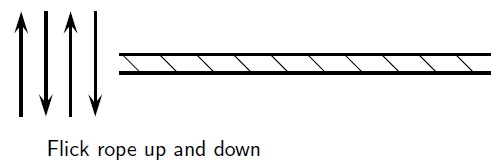
\includegraphics[width=300px]{col11305.imgs/m38806_PG10C5_001.png} % m38806;PG10C5\_001.png;;;6.0;8.5;
        
      \vspace{2pt}
    \vspace{.1in}
    
    \end{center}

 \end{figure}   

    \addtocounter{footnote}{-0}
    
      \par 
      \label{m38806*id317791}\begin{enumerate}[noitemsep, label=\textbf{\arabic*}. ] 
            \label{m38806*uid1}\item Describe what happens to the rope.
\label{m38806*uid2}\item Draw a diagram of what the rope looks like while the pulses travel along it.
\label{m38806*uid3}\item In which direction do the pulses travel?
\label{m38806*uid4}\item Tie a ribbon to the middle of the rope. This indicates a particle in the rope.

    \setcounter{subfigure}{0}


	\begin{figure}[H] % horizontal\label{m38806*id317844}
    \begin{center}
    \label{m38806*id317844!!!underscore!!!media}\label{m38806*id317844!!!underscore!!!printimage}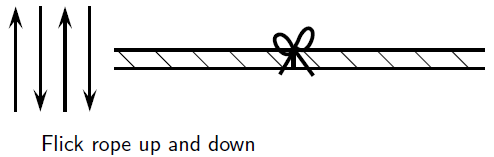
\includegraphics[width=300px]{col11305.imgs/m38806_PG10C5_002.png} % m38806;PG10C5\_002.png;;;6.0;8.5;
        
      \vspace{2pt}
    \vspace{.1in}
    
    \end{center}

 \end{figure}   

    \addtocounter{footnote}{-0}
    \label{m38806*uid5}\item Flick the rope continuously. Watch the ribbon carefully as the pulses travel through the rope. What happens to the ribbon?
\label{m38806*uid6}\item Draw a picture to show the motion of the ribbon. Draw the ribbon as a dot and use arrows to indicate how it moves.
\end{enumerate}
        
      

      \label{m38806*id317884}In the Activity, you have created waves. The medium through which these waves propagated was the rope, which is obviously made up of a very large number of particles (atoms).
From the activity, you would have noticed that the wave travelled from left to right, but the particles (the ribbon) moved only up and down.\par 
      
    \setcounter{subfigure}{0}


	\begin{figure}[H] % horizontal\label{m38806*uid7}
    \begin{center}
    \rule[.1in]{\figurerulewidth}{.005in} \\
        \label{m38806*uid7!!!underscore!!!media}\label{m38806*uid7!!!underscore!!!printimage}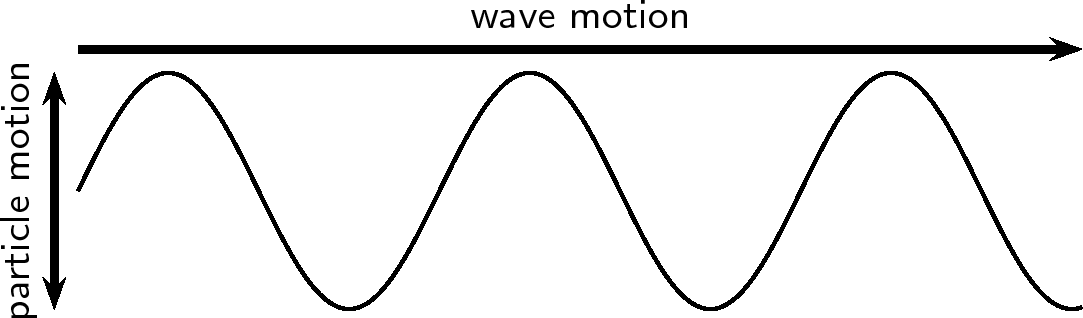
\includegraphics[width=300px]{col11305.imgs/m38806_PG10C5_003.png} % m38806;PG10C5\_003.png;;;6.0;8.5;
        
      \vspace{2pt}
    \vspace{\rubberspace}\par \begin{cnxcaption}
	  \small \textbf{Figure 7.3: }A transverse wave, showing the direction of motion of the wave perpendicular to the direction in which the particles move.
	\end{cnxcaption}
      
    \vspace{.1in}
    \rule[.1in]{\figurerulewidth}{.005in} \\
        
    \end{center}

 \end{figure}   

    \addtocounter{footnote}{-0}
    
      \label{m38806*id317903}When the particles of a medium move at right angles to the direction of propagation of a wave, the wave is called \textsl{transverse}. For waves, there is no net displacement of the particles (they return to their equilibrium position), but there is a net displacement of the wave. There are thus two different motions: the motion of the particles of the medium and the motion of the wave.\par 
      \label{m38806*eip-375}The following simulation will help you understand more about waves. Select the oscillate option and then observe what happens.

    \setcounter{subfigure}{0}


	\begin{figure}[H] % horizontal\label{m38806*transverse-waves}
    
    
    \textnormal{Phet simulation for Transverse Waves}\vspace{.1in} \nopagebreak
  \label{m38806*phet!!!underscore!!!sim}\label{m38806*phet-simulation}
            \raisebox{-5 pt}{ 
\includegraphics[width=0.5cm]{col11305.imgs/summary_www.png}} { (Simulation:  P10042 )}
      
      \vspace{2pt}
    \vspace{.1in}
    
    

 \end{figure}   

    \addtocounter{footnote}{-0}
    \par \label{m38806*uid8}
            \subsection{ Peaks and Troughs}
            \nopagebreak
            
        
        \label{m38806*id317923}Waves have moving \textsl{peaks} (or \textsl{crests}) and \textsl{troughs}. A peak is the highest point the medium rises to and a trough is the lowest point the medium sinks to.\par 
        \label{m38806*id317942}Peaks and troughs on a transverse wave are shown in Figure~7.5.\par 
        
    \setcounter{subfigure}{0}


	\begin{figure}[H] % horizontal\label{m38806*uid9}
    \begin{center}
    \rule[.1in]{\figurerulewidth}{.005in} \\
        \label{m38806*uid9!!!underscore!!!media}\label{m38806*uid9!!!underscore!!!printimage}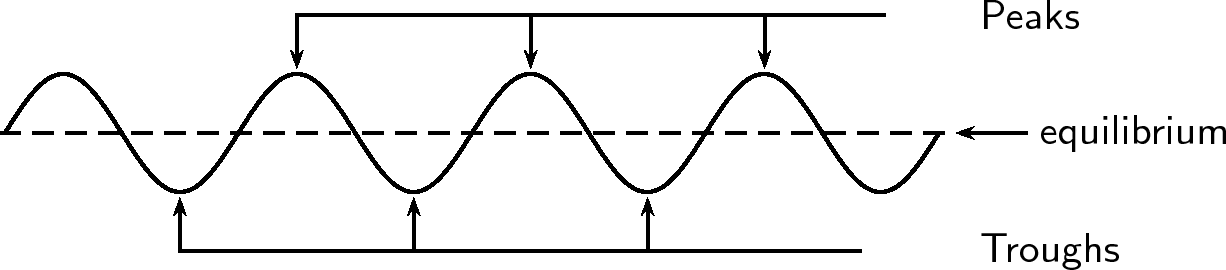
\includegraphics[width=300px]{col11305.imgs/m38806_PG10C5_004.png} % m38806;PG10C5\_004.png;;;6.0;8.5;
        
      \vspace{2pt}
    \vspace{\rubberspace}\par \begin{cnxcaption}
	  \small \textbf{Figure 7.5: }Peaks and troughs in a transverse wave.
	\end{cnxcaption}
      
    \vspace{.1in}
    \rule[.1in]{\figurerulewidth}{.005in} \\
        
    \end{center}

 \end{figure}   

    \addtocounter{footnote}{-0}
    
\par
            \label{m38806*fhsst!!!underscore!!!id136}\begin{definition}
	  \begin{tabular*}{15 cm}{m{15 mm}m{}}
	\hspace*{-50pt}  
\includegraphics[width=0.5in]{col11305.imgs/psflag2.png}   & \Definition{   \label{id2439255}\textbf{ Peaks and troughs }} { \label{m38806*meaningfhsst!!!underscore!!!id136}
        \label{m38806*id317968}A \textsl{peak} is a point on the wave where the displacement of the medium is at a maximum. A point on the wave is a \textsl{trough} if the displacement of the medium at that point is at a minimum.  \par 
         } 
      \end{tabular*}
      \end{definition}

      
      \label{m38806*uid10}
            \subsection{ Amplitude and Wavelength}
            \nopagebreak
            
        
        \label{m38806*id318000}There are a few properties that we saw with pulses that also apply to waves. These are amplitude and wavelength (we called this pulse length).\par 
\label{m38806*fhsst!!!underscore!!!id143}\begin{definition}
	  \begin{tabular*}{15 cm}{m{15 mm}m{}}
	\hspace*{-50pt}  
\includegraphics[width=0.5in]{col11305.imgs/psflag2.png}   & \Definition{   \label{id2439313}\textbf{ Amplitude }} { \label{m38806*meaningfhsst!!!underscore!!!id143}
        \label{m38806*id318011}The \textsl{amplitude} is the maximum displacement of a particle from its equilibrium position. \par 
         } 
      \end{tabular*}
      \end{definition}

\label{m38806*secfhsst!!!underscore!!!id146}
            \subsubsection{  Investigation : Amplitude }
            \nopagebreak
            
        \label{m38806*id318034}
    \setcounter{subfigure}{0}


	\begin{figure}[H] % horizontal\label{m38806*id318037}
    \begin{center}
    \label{m38806*id318037!!!underscore!!!media}\label{m38806*id318037!!!underscore!!!printimage}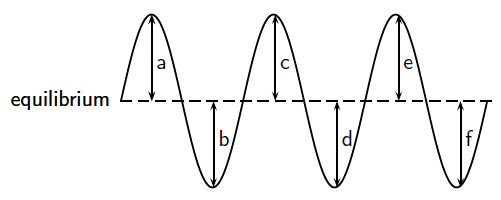
\includegraphics[width=300px]{col11305.imgs/m38806_PG10C5_005.png} % m38806;PG10C5\_005.png;;;6.0;8.5;
        
      \vspace{2pt}
    \vspace{.1in}
    
    \end{center}

 \end{figure}   

    \addtocounter{footnote}{-0}
    
        \par 
        \label{m38806*id318043}Fill in the table below by measuring the distance between the equilibrium and each peak and troughs in the wave above. Use your ruler to measure the distances.\par 
        
    % \textbf{m38806*id318048}\par
    
    % how many colspecs?  2
          % name: cnx:colspec
            % colnum: 1
            % colwidth: 10*
            % latex-name: columna
            % colname: 
            % align/tgroup-align/default: //left
            % -------------------------
            % name: cnx:colspec
            % colnum: 2
            % colwidth: 10*
            % latex-name: columnb
            % colname: 
            % align/tgroup-align/default: //left
            % -------------------------
      
    
    \setlength\mytablespace{4\tabcolsep}
    \addtolength\mytablespace{3\arrayrulewidth}
    \setlength\mytablewidth{\linewidth}
        
    
    \setlength\mytableroom{\mytablewidth}
    \addtolength\mytableroom{-\mytablespace}
    
    \setlength\myfixedwidth{0pt}
    \setlength\mystarwidth{\mytableroom}
        \addtolength\mystarwidth{-\myfixedwidth}
        \divide\mystarwidth 20
        
    
      % ----- Begin capturing width of table in LR mode woof
      \settowidth{\mytableboxwidth}{\begin{tabular}[t]{|l|l|}\hline
    % count in rowspan-info-nodeset: 2
    % align/colidx: left,1
    
    % rowcount: '0' | start: 'false' | colidx: '1'
    
        % Formatting a regular cell and recurring on the next sibling
        Peak/Trough &
      % align/colidx: left,2
    
    % rowcount: '0' | start: 'false' | colidx: '2'
    
        % Formatting a regular cell and recurring on the next sibling
        Measurement (cm)% make-rowspan-placeholders
    % rowspan info: col1 '0' | 'false' | '' || col2 '0' | 'false' | ''
     \tabularnewline\cline{1-1}\cline{2-2}
      %--------------------------------------------------------------------
    % align/colidx: left,1
    
    % rowcount: '0' | start: 'false' | colidx: '1'
    
        % Formatting a regular cell and recurring on the next sibling
        a &
      % align/colidx: left,2
    
    % rowcount: '0' | start: 'false' | colidx: '2'
    
        % Formatting a regular cell and recurring on the next sibling
        % make-rowspan-placeholders
    % rowspan info: col1 '0' | 'false' | '' || col2 '0' | 'false' | ''
     \tabularnewline\cline{1-1}\cline{2-2}
      %--------------------------------------------------------------------
    % align/colidx: left,1
    
    % rowcount: '0' | start: 'false' | colidx: '1'
    
        % Formatting a regular cell and recurring on the next sibling
        b &
      % align/colidx: left,2
    
    % rowcount: '0' | start: 'false' | colidx: '2'
    
        % Formatting a regular cell and recurring on the next sibling
        % make-rowspan-placeholders
    % rowspan info: col1 '0' | 'false' | '' || col2 '0' | 'false' | ''
     \tabularnewline\cline{1-1}\cline{2-2}
      %--------------------------------------------------------------------
    % align/colidx: left,1
    
    % rowcount: '0' | start: 'false' | colidx: '1'
    
        % Formatting a regular cell and recurring on the next sibling
        c &
      % align/colidx: left,2
    
    % rowcount: '0' | start: 'false' | colidx: '2'
    
        % Formatting a regular cell and recurring on the next sibling
        % make-rowspan-placeholders
    % rowspan info: col1 '0' | 'false' | '' || col2 '0' | 'false' | ''
     \tabularnewline\cline{1-1}\cline{2-2}
      %--------------------------------------------------------------------
    % align/colidx: left,1
    
    % rowcount: '0' | start: 'false' | colidx: '1'
    
        % Formatting a regular cell and recurring on the next sibling
        d &
      % align/colidx: left,2
    
    % rowcount: '0' | start: 'false' | colidx: '2'
    
        % Formatting a regular cell and recurring on the next sibling
        % make-rowspan-placeholders
    % rowspan info: col1 '0' | 'false' | '' || col2 '0' | 'false' | ''
     \tabularnewline\cline{1-1}\cline{2-2}
      %--------------------------------------------------------------------
    % align/colidx: left,1
    
    % rowcount: '0' | start: 'false' | colidx: '1'
    
        % Formatting a regular cell and recurring on the next sibling
        e &
      % align/colidx: left,2
    
    % rowcount: '0' | start: 'false' | colidx: '2'
    
        % Formatting a regular cell and recurring on the next sibling
        % make-rowspan-placeholders
    % rowspan info: col1 '0' | 'false' | '' || col2 '0' | 'false' | ''
     \tabularnewline\cline{1-1}\cline{2-2}
      %--------------------------------------------------------------------
    % align/colidx: left,1
    
    % rowcount: '0' | start: 'false' | colidx: '1'
    
        % Formatting a regular cell and recurring on the next sibling
        f &
      % align/colidx: left,2
    
    % rowcount: '0' | start: 'false' | colidx: '2'
    
        % Formatting a regular cell and recurring on the next sibling
        % make-rowspan-placeholders
    % rowspan info: col1 '0' | 'false' | '' || col2 '0' | 'false' | ''
     \tabularnewline\cline{1-1}\cline{2-2}
      %--------------------------------------------------------------------
    \end{tabular}} % end mytableboxwidth set
      \addtocounter{footnote}{-0}
      
      % ----- End capturing width of table in LR mode
    
        % ----- LR or paragraph mode: must test
        % ----- Begin capturing height of table
        \settoheight{\mytableboxheight}{\begin{tabular}[t]{|l|l|}\hline
    % count in rowspan-info-nodeset: 2
    % align/colidx: left,1
    
    % rowcount: '0' | start: 'false' | colidx: '1'
    
        % Formatting a regular cell and recurring on the next sibling
        Peak/Trough &
      % align/colidx: left,2
    
    % rowcount: '0' | start: 'false' | colidx: '2'
    
        % Formatting a regular cell and recurring on the next sibling
        Measurement (cm)% make-rowspan-placeholders
    % rowspan info: col1 '0' | 'false' | '' || col2 '0' | 'false' | ''
     \tabularnewline\cline{1-1}\cline{2-2}
      %--------------------------------------------------------------------
    % align/colidx: left,1
    
    % rowcount: '0' | start: 'false' | colidx: '1'
    
        % Formatting a regular cell and recurring on the next sibling
        a &
      % align/colidx: left,2
    
    % rowcount: '0' | start: 'false' | colidx: '2'
    
        % Formatting a regular cell and recurring on the next sibling
        % make-rowspan-placeholders
    % rowspan info: col1 '0' | 'false' | '' || col2 '0' | 'false' | ''
     \tabularnewline\cline{1-1}\cline{2-2}
      %--------------------------------------------------------------------
    % align/colidx: left,1
    
    % rowcount: '0' | start: 'false' | colidx: '1'
    
        % Formatting a regular cell and recurring on the next sibling
        b &
      % align/colidx: left,2
    
    % rowcount: '0' | start: 'false' | colidx: '2'
    
        % Formatting a regular cell and recurring on the next sibling
        % make-rowspan-placeholders
    % rowspan info: col1 '0' | 'false' | '' || col2 '0' | 'false' | ''
     \tabularnewline\cline{1-1}\cline{2-2}
      %--------------------------------------------------------------------
    % align/colidx: left,1
    
    % rowcount: '0' | start: 'false' | colidx: '1'
    
        % Formatting a regular cell and recurring on the next sibling
        c &
      % align/colidx: left,2
    
    % rowcount: '0' | start: 'false' | colidx: '2'
    
        % Formatting a regular cell and recurring on the next sibling
        % make-rowspan-placeholders
    % rowspan info: col1 '0' | 'false' | '' || col2 '0' | 'false' | ''
     \tabularnewline\cline{1-1}\cline{2-2}
      %--------------------------------------------------------------------
    % align/colidx: left,1
    
    % rowcount: '0' | start: 'false' | colidx: '1'
    
        % Formatting a regular cell and recurring on the next sibling
        d &
      % align/colidx: left,2
    
    % rowcount: '0' | start: 'false' | colidx: '2'
    
        % Formatting a regular cell and recurring on the next sibling
        % make-rowspan-placeholders
    % rowspan info: col1 '0' | 'false' | '' || col2 '0' | 'false' | ''
     \tabularnewline\cline{1-1}\cline{2-2}
      %--------------------------------------------------------------------
    % align/colidx: left,1
    
    % rowcount: '0' | start: 'false' | colidx: '1'
    
        % Formatting a regular cell and recurring on the next sibling
        e &
      % align/colidx: left,2
    
    % rowcount: '0' | start: 'false' | colidx: '2'
    
        % Formatting a regular cell and recurring on the next sibling
        % make-rowspan-placeholders
    % rowspan info: col1 '0' | 'false' | '' || col2 '0' | 'false' | ''
     \tabularnewline\cline{1-1}\cline{2-2}
      %--------------------------------------------------------------------
    % align/colidx: left,1
    
    % rowcount: '0' | start: 'false' | colidx: '1'
    
        % Formatting a regular cell and recurring on the next sibling
        f &
      % align/colidx: left,2
    
    % rowcount: '0' | start: 'false' | colidx: '2'
    
        % Formatting a regular cell and recurring on the next sibling
        % make-rowspan-placeholders
    % rowspan info: col1 '0' | 'false' | '' || col2 '0' | 'false' | ''
     \tabularnewline\cline{1-1}\cline{2-2}
      %--------------------------------------------------------------------
    \end{tabular}} % end mytableboxheight set
        \settodepth{\mytableboxdepth}{\begin{tabular}[t]{|l|l|}\hline
    % count in rowspan-info-nodeset: 2
    % align/colidx: left,1
    
    % rowcount: '0' | start: 'false' | colidx: '1'
    
        % Formatting a regular cell and recurring on the next sibling
        Peak/Trough &
      % align/colidx: left,2
    
    % rowcount: '0' | start: 'false' | colidx: '2'
    
        % Formatting a regular cell and recurring on the next sibling
        Measurement (cm)% make-rowspan-placeholders
    % rowspan info: col1 '0' | 'false' | '' || col2 '0' | 'false' | ''
     \tabularnewline\cline{1-1}\cline{2-2}
      %--------------------------------------------------------------------
    % align/colidx: left,1
    
    % rowcount: '0' | start: 'false' | colidx: '1'
    
        % Formatting a regular cell and recurring on the next sibling
        a &
      % align/colidx: left,2
    
    % rowcount: '0' | start: 'false' | colidx: '2'
    
        % Formatting a regular cell and recurring on the next sibling
        % make-rowspan-placeholders
    % rowspan info: col1 '0' | 'false' | '' || col2 '0' | 'false' | ''
     \tabularnewline\cline{1-1}\cline{2-2}
      %--------------------------------------------------------------------
    % align/colidx: left,1
    
    % rowcount: '0' | start: 'false' | colidx: '1'
    
        % Formatting a regular cell and recurring on the next sibling
        b &
      % align/colidx: left,2
    
    % rowcount: '0' | start: 'false' | colidx: '2'
    
        % Formatting a regular cell and recurring on the next sibling
        % make-rowspan-placeholders
    % rowspan info: col1 '0' | 'false' | '' || col2 '0' | 'false' | ''
     \tabularnewline\cline{1-1}\cline{2-2}
      %--------------------------------------------------------------------
    % align/colidx: left,1
    
    % rowcount: '0' | start: 'false' | colidx: '1'
    
        % Formatting a regular cell and recurring on the next sibling
        c &
      % align/colidx: left,2
    
    % rowcount: '0' | start: 'false' | colidx: '2'
    
        % Formatting a regular cell and recurring on the next sibling
        % make-rowspan-placeholders
    % rowspan info: col1 '0' | 'false' | '' || col2 '0' | 'false' | ''
     \tabularnewline\cline{1-1}\cline{2-2}
      %--------------------------------------------------------------------
    % align/colidx: left,1
    
    % rowcount: '0' | start: 'false' | colidx: '1'
    
        % Formatting a regular cell and recurring on the next sibling
        d &
      % align/colidx: left,2
    
    % rowcount: '0' | start: 'false' | colidx: '2'
    
        % Formatting a regular cell and recurring on the next sibling
        % make-rowspan-placeholders
    % rowspan info: col1 '0' | 'false' | '' || col2 '0' | 'false' | ''
     \tabularnewline\cline{1-1}\cline{2-2}
      %--------------------------------------------------------------------
    % align/colidx: left,1
    
    % rowcount: '0' | start: 'false' | colidx: '1'
    
        % Formatting a regular cell and recurring on the next sibling
        e &
      % align/colidx: left,2
    
    % rowcount: '0' | start: 'false' | colidx: '2'
    
        % Formatting a regular cell and recurring on the next sibling
        % make-rowspan-placeholders
    % rowspan info: col1 '0' | 'false' | '' || col2 '0' | 'false' | ''
     \tabularnewline\cline{1-1}\cline{2-2}
      %--------------------------------------------------------------------
    % align/colidx: left,1
    
    % rowcount: '0' | start: 'false' | colidx: '1'
    
        % Formatting a regular cell and recurring on the next sibling
        f &
      % align/colidx: left,2
    
    % rowcount: '0' | start: 'false' | colidx: '2'
    
        % Formatting a regular cell and recurring on the next sibling
        % make-rowspan-placeholders
    % rowspan info: col1 '0' | 'false' | '' || col2 '0' | 'false' | ''
     \tabularnewline\cline{1-1}\cline{2-2}
      %--------------------------------------------------------------------
    \end{tabular}} % end mytableboxdepth set
        \addtolength{\mytableboxheight}{\mytableboxdepth}
        % ----- End capturing height of table
        \addtocounter{footnote}{-0}
        
        \ifthenelse{\mytableboxwidth<\textwidth}{% the table fits in LR mode
          \addtolength{\mytableboxwidth}{-\mytablespace}
          \typeout{textheight: \the\textheight}
          \typeout{mytableboxheight: \the\mytableboxheight}
          \typeout{textwidth: \the\textwidth}
          \typeout{mytableboxwidth: \the\mytableboxwidth}
          \ifthenelse{\mytableboxheight<\textheight}{%
        
    % \begin{table}[H]
    % \\ '' '0'
    
        \begin{center}
      
      \label{m38806*id318048}
      
    \noindent
    \begin{tabular}[t]{|l|l|}\hline
    % count in rowspan-info-nodeset: 2
    % align/colidx: left,1
    
    % rowcount: '0' | start: 'false' | colidx: '1'
    
        % Formatting a regular cell and recurring on the next sibling
        Peak/Trough &
      % align/colidx: left,2
    
    % rowcount: '0' | start: 'false' | colidx: '2'
    
        % Formatting a regular cell and recurring on the next sibling
        Measurement (cm)% make-rowspan-placeholders
    % rowspan info: col1 '0' | 'false' | '' || col2 '0' | 'false' | ''
     \tabularnewline\cline{1-1}\cline{2-2}
      %--------------------------------------------------------------------
    % align/colidx: left,1
    
    % rowcount: '0' | start: 'false' | colidx: '1'
    
        % Formatting a regular cell and recurring on the next sibling
        a &
      % align/colidx: left,2
    
    % rowcount: '0' | start: 'false' | colidx: '2'
    
        % Formatting a regular cell and recurring on the next sibling
        % make-rowspan-placeholders
    % rowspan info: col1 '0' | 'false' | '' || col2 '0' | 'false' | ''
     \tabularnewline\cline{1-1}\cline{2-2}
      %--------------------------------------------------------------------
    % align/colidx: left,1
    
    % rowcount: '0' | start: 'false' | colidx: '1'
    
        % Formatting a regular cell and recurring on the next sibling
        b &
      % align/colidx: left,2
    
    % rowcount: '0' | start: 'false' | colidx: '2'
    
        % Formatting a regular cell and recurring on the next sibling
        % make-rowspan-placeholders
    % rowspan info: col1 '0' | 'false' | '' || col2 '0' | 'false' | ''
     \tabularnewline\cline{1-1}\cline{2-2}
      %--------------------------------------------------------------------
    % align/colidx: left,1
    
    % rowcount: '0' | start: 'false' | colidx: '1'
    
        % Formatting a regular cell and recurring on the next sibling
        c &
      % align/colidx: left,2
    
    % rowcount: '0' | start: 'false' | colidx: '2'
    
        % Formatting a regular cell and recurring on the next sibling
        % make-rowspan-placeholders
    % rowspan info: col1 '0' | 'false' | '' || col2 '0' | 'false' | ''
     \tabularnewline\cline{1-1}\cline{2-2}
      %--------------------------------------------------------------------
    % align/colidx: left,1
    
    % rowcount: '0' | start: 'false' | colidx: '1'
    
        % Formatting a regular cell and recurring on the next sibling
        d &
      % align/colidx: left,2
    
    % rowcount: '0' | start: 'false' | colidx: '2'
    
        % Formatting a regular cell and recurring on the next sibling
        % make-rowspan-placeholders
    % rowspan info: col1 '0' | 'false' | '' || col2 '0' | 'false' | ''
     \tabularnewline\cline{1-1}\cline{2-2}
      %--------------------------------------------------------------------
    % align/colidx: left,1
    
    % rowcount: '0' | start: 'false' | colidx: '1'
    
        % Formatting a regular cell and recurring on the next sibling
        e &
      % align/colidx: left,2
    
    % rowcount: '0' | start: 'false' | colidx: '2'
    
        % Formatting a regular cell and recurring on the next sibling
        % make-rowspan-placeholders
    % rowspan info: col1 '0' | 'false' | '' || col2 '0' | 'false' | ''
     \tabularnewline\cline{1-1}\cline{2-2}
      %--------------------------------------------------------------------
    % align/colidx: left,1
    
    % rowcount: '0' | start: 'false' | colidx: '1'
    
        % Formatting a regular cell and recurring on the next sibling
        f &
      % align/colidx: left,2
    
    % rowcount: '0' | start: 'false' | colidx: '2'
    
        % Formatting a regular cell and recurring on the next sibling
        % make-rowspan-placeholders
    % rowspan info: col1 '0' | 'false' | '' || col2 '0' | 'false' | ''
     \tabularnewline\cline{1-1}\cline{2-2}
      %--------------------------------------------------------------------
    \end{tabular}
      \end{center}
    \begin{center}{\small\bfseries Table 7.1}\end{center}
    %\end{table}
    
    \addtocounter{footnote}{-0}
    
          }{ % else
        
    % \begin{table}[H]
    % \\ '' '0'
    
        \begin{center}
      
      \label{m38806*id318048}
      
    \noindent
    \tabletail{%
        \hline
        \multicolumn{2}{|p{\mytableboxwidth}|}{\raggedleft \small \sl continued on next page}\\
        \hline
      }
      \tablelasttail{}
      \begin{xtabular}[t]{|l|l|}\hline
    % count in rowspan-info-nodeset: 2
    % align/colidx: left,1
    
    % rowcount: '0' | start: 'false' | colidx: '1'
    
        % Formatting a regular cell and recurring on the next sibling
        Peak/Trough &
      % align/colidx: left,2
    
    % rowcount: '0' | start: 'false' | colidx: '2'
    
        % Formatting a regular cell and recurring on the next sibling
        Measurement (cm)% make-rowspan-placeholders
    % rowspan info: col1 '0' | 'false' | '' || col2 '0' | 'false' | ''
     \tabularnewline\cline{1-1}\cline{2-2}
      %--------------------------------------------------------------------
    % align/colidx: left,1
    
    % rowcount: '0' | start: 'false' | colidx: '1'
    
        % Formatting a regular cell and recurring on the next sibling
        a &
      % align/colidx: left,2
    
    % rowcount: '0' | start: 'false' | colidx: '2'
    
        % Formatting a regular cell and recurring on the next sibling
        % make-rowspan-placeholders
    % rowspan info: col1 '0' | 'false' | '' || col2 '0' | 'false' | ''
     \tabularnewline\cline{1-1}\cline{2-2}
      %--------------------------------------------------------------------
    % align/colidx: left,1
    
    % rowcount: '0' | start: 'false' | colidx: '1'
    
        % Formatting a regular cell and recurring on the next sibling
        b &
      % align/colidx: left,2
    
    % rowcount: '0' | start: 'false' | colidx: '2'
    
        % Formatting a regular cell and recurring on the next sibling
        % make-rowspan-placeholders
    % rowspan info: col1 '0' | 'false' | '' || col2 '0' | 'false' | ''
     \tabularnewline\cline{1-1}\cline{2-2}
      %--------------------------------------------------------------------
    % align/colidx: left,1
    
    % rowcount: '0' | start: 'false' | colidx: '1'
    
        % Formatting a regular cell and recurring on the next sibling
        c &
      % align/colidx: left,2
    
    % rowcount: '0' | start: 'false' | colidx: '2'
    
        % Formatting a regular cell and recurring on the next sibling
        % make-rowspan-placeholders
    % rowspan info: col1 '0' | 'false' | '' || col2 '0' | 'false' | ''
     \tabularnewline\cline{1-1}\cline{2-2}
      %--------------------------------------------------------------------
    % align/colidx: left,1
    
    % rowcount: '0' | start: 'false' | colidx: '1'
    
        % Formatting a regular cell and recurring on the next sibling
        d &
      % align/colidx: left,2
    
    % rowcount: '0' | start: 'false' | colidx: '2'
    
        % Formatting a regular cell and recurring on the next sibling
        % make-rowspan-placeholders
    % rowspan info: col1 '0' | 'false' | '' || col2 '0' | 'false' | ''
     \tabularnewline\cline{1-1}\cline{2-2}
      %--------------------------------------------------------------------
    % align/colidx: left,1
    
    % rowcount: '0' | start: 'false' | colidx: '1'
    
        % Formatting a regular cell and recurring on the next sibling
        e &
      % align/colidx: left,2
    
    % rowcount: '0' | start: 'false' | colidx: '2'
    
        % Formatting a regular cell and recurring on the next sibling
        % make-rowspan-placeholders
    % rowspan info: col1 '0' | 'false' | '' || col2 '0' | 'false' | ''
     \tabularnewline\cline{1-1}\cline{2-2}
      %--------------------------------------------------------------------
    % align/colidx: left,1
    
    % rowcount: '0' | start: 'false' | colidx: '1'
    
        % Formatting a regular cell and recurring on the next sibling
        f &
      % align/colidx: left,2
    
    % rowcount: '0' | start: 'false' | colidx: '2'
    
        % Formatting a regular cell and recurring on the next sibling
        % make-rowspan-placeholders
    % rowspan info: col1 '0' | 'false' | '' || col2 '0' | 'false' | ''
     \tabularnewline\cline{1-1}\cline{2-2}
      %--------------------------------------------------------------------
    \end{xtabular}
      \end{center}
    \begin{center}{\small\bfseries Table 7.1}\end{center}
    %\end{table}
    
    \addtocounter{footnote}{-0}
    
          } % 
        }{% else
        % typeset the table in paragraph mode
        % ----- Begin capturing height of table
        \settoheight{\mytableboxheight}{\begin{tabular*}{\mytablewidth}[t]{|p{10\mystarwidth}|p{10\mystarwidth}|}\hline
    % count in rowspan-info-nodeset: 2
    % align/colidx: left,1
    
    % rowcount: '0' | start: 'false' | colidx: '1'
    
        % Formatting a regular cell and recurring on the next sibling
        Peak/Trough &
      % align/colidx: left,2
    
    % rowcount: '0' | start: 'false' | colidx: '2'
    
        % Formatting a regular cell and recurring on the next sibling
        Measurement (cm)% make-rowspan-placeholders
    % rowspan info: col1 '0' | 'false' | '' || col2 '0' | 'false' | ''
     \tabularnewline\cline{1-1}\cline{2-2}
      %--------------------------------------------------------------------
    % align/colidx: left,1
    
    % rowcount: '0' | start: 'false' | colidx: '1'
    
        % Formatting a regular cell and recurring on the next sibling
        a &
      % align/colidx: left,2
    
    % rowcount: '0' | start: 'false' | colidx: '2'
    
        % Formatting a regular cell and recurring on the next sibling
        % make-rowspan-placeholders
    % rowspan info: col1 '0' | 'false' | '' || col2 '0' | 'false' | ''
     \tabularnewline\cline{1-1}\cline{2-2}
      %--------------------------------------------------------------------
    % align/colidx: left,1
    
    % rowcount: '0' | start: 'false' | colidx: '1'
    
        % Formatting a regular cell and recurring on the next sibling
        b &
      % align/colidx: left,2
    
    % rowcount: '0' | start: 'false' | colidx: '2'
    
        % Formatting a regular cell and recurring on the next sibling
        % make-rowspan-placeholders
    % rowspan info: col1 '0' | 'false' | '' || col2 '0' | 'false' | ''
     \tabularnewline\cline{1-1}\cline{2-2}
      %--------------------------------------------------------------------
    % align/colidx: left,1
    
    % rowcount: '0' | start: 'false' | colidx: '1'
    
        % Formatting a regular cell and recurring on the next sibling
        c &
      % align/colidx: left,2
    
    % rowcount: '0' | start: 'false' | colidx: '2'
    
        % Formatting a regular cell and recurring on the next sibling
        % make-rowspan-placeholders
    % rowspan info: col1 '0' | 'false' | '' || col2 '0' | 'false' | ''
     \tabularnewline\cline{1-1}\cline{2-2}
      %--------------------------------------------------------------------
    % align/colidx: left,1
    
    % rowcount: '0' | start: 'false' | colidx: '1'
    
        % Formatting a regular cell and recurring on the next sibling
        d &
      % align/colidx: left,2
    
    % rowcount: '0' | start: 'false' | colidx: '2'
    
        % Formatting a regular cell and recurring on the next sibling
        % make-rowspan-placeholders
    % rowspan info: col1 '0' | 'false' | '' || col2 '0' | 'false' | ''
     \tabularnewline\cline{1-1}\cline{2-2}
      %--------------------------------------------------------------------
    % align/colidx: left,1
    
    % rowcount: '0' | start: 'false' | colidx: '1'
    
        % Formatting a regular cell and recurring on the next sibling
        e &
      % align/colidx: left,2
    
    % rowcount: '0' | start: 'false' | colidx: '2'
    
        % Formatting a regular cell and recurring on the next sibling
        % make-rowspan-placeholders
    % rowspan info: col1 '0' | 'false' | '' || col2 '0' | 'false' | ''
     \tabularnewline\cline{1-1}\cline{2-2}
      %--------------------------------------------------------------------
    % align/colidx: left,1
    
    % rowcount: '0' | start: 'false' | colidx: '1'
    
        % Formatting a regular cell and recurring on the next sibling
        f &
      % align/colidx: left,2
    
    % rowcount: '0' | start: 'false' | colidx: '2'
    
        % Formatting a regular cell and recurring on the next sibling
        % make-rowspan-placeholders
    % rowspan info: col1 '0' | 'false' | '' || col2 '0' | 'false' | ''
     \tabularnewline\cline{1-1}\cline{2-2}
      %--------------------------------------------------------------------
    \end{tabular*}} % end mytableboxheight set
        \settodepth{\mytableboxdepth}{\begin{tabular*}{\mytablewidth}[t]{|p{10\mystarwidth}|p{10\mystarwidth}|}\hline
    % count in rowspan-info-nodeset: 2
    % align/colidx: left,1
    
    % rowcount: '0' | start: 'false' | colidx: '1'
    
        % Formatting a regular cell and recurring on the next sibling
        Peak/Trough &
      % align/colidx: left,2
    
    % rowcount: '0' | start: 'false' | colidx: '2'
    
        % Formatting a regular cell and recurring on the next sibling
        Measurement (cm)% make-rowspan-placeholders
    % rowspan info: col1 '0' | 'false' | '' || col2 '0' | 'false' | ''
     \tabularnewline\cline{1-1}\cline{2-2}
      %--------------------------------------------------------------------
    % align/colidx: left,1
    
    % rowcount: '0' | start: 'false' | colidx: '1'
    
        % Formatting a regular cell and recurring on the next sibling
        a &
      % align/colidx: left,2
    
    % rowcount: '0' | start: 'false' | colidx: '2'
    
        % Formatting a regular cell and recurring on the next sibling
        % make-rowspan-placeholders
    % rowspan info: col1 '0' | 'false' | '' || col2 '0' | 'false' | ''
     \tabularnewline\cline{1-1}\cline{2-2}
      %--------------------------------------------------------------------
    % align/colidx: left,1
    
    % rowcount: '0' | start: 'false' | colidx: '1'
    
        % Formatting a regular cell and recurring on the next sibling
        b &
      % align/colidx: left,2
    
    % rowcount: '0' | start: 'false' | colidx: '2'
    
        % Formatting a regular cell and recurring on the next sibling
        % make-rowspan-placeholders
    % rowspan info: col1 '0' | 'false' | '' || col2 '0' | 'false' | ''
     \tabularnewline\cline{1-1}\cline{2-2}
      %--------------------------------------------------------------------
    % align/colidx: left,1
    
    % rowcount: '0' | start: 'false' | colidx: '1'
    
        % Formatting a regular cell and recurring on the next sibling
        c &
      % align/colidx: left,2
    
    % rowcount: '0' | start: 'false' | colidx: '2'
    
        % Formatting a regular cell and recurring on the next sibling
        % make-rowspan-placeholders
    % rowspan info: col1 '0' | 'false' | '' || col2 '0' | 'false' | ''
     \tabularnewline\cline{1-1}\cline{2-2}
      %--------------------------------------------------------------------
    % align/colidx: left,1
    
    % rowcount: '0' | start: 'false' | colidx: '1'
    
        % Formatting a regular cell and recurring on the next sibling
        d &
      % align/colidx: left,2
    
    % rowcount: '0' | start: 'false' | colidx: '2'
    
        % Formatting a regular cell and recurring on the next sibling
        % make-rowspan-placeholders
    % rowspan info: col1 '0' | 'false' | '' || col2 '0' | 'false' | ''
     \tabularnewline\cline{1-1}\cline{2-2}
      %--------------------------------------------------------------------
    % align/colidx: left,1
    
    % rowcount: '0' | start: 'false' | colidx: '1'
    
        % Formatting a regular cell and recurring on the next sibling
        e &
      % align/colidx: left,2
    
    % rowcount: '0' | start: 'false' | colidx: '2'
    
        % Formatting a regular cell and recurring on the next sibling
        % make-rowspan-placeholders
    % rowspan info: col1 '0' | 'false' | '' || col2 '0' | 'false' | ''
     \tabularnewline\cline{1-1}\cline{2-2}
      %--------------------------------------------------------------------
    % align/colidx: left,1
    
    % rowcount: '0' | start: 'false' | colidx: '1'
    
        % Formatting a regular cell and recurring on the next sibling
        f &
      % align/colidx: left,2
    
    % rowcount: '0' | start: 'false' | colidx: '2'
    
        % Formatting a regular cell and recurring on the next sibling
        % make-rowspan-placeholders
    % rowspan info: col1 '0' | 'false' | '' || col2 '0' | 'false' | ''
     \tabularnewline\cline{1-1}\cline{2-2}
      %--------------------------------------------------------------------
    \end{tabular*}} % end mytableboxdepth set
        \addtolength{\mytableboxheight}{\mytableboxdepth}
        % ----- End capturing height of table
        \typeout{textheight: \the\textheight}
        \typeout{mytableboxheight: \the\mytableboxheight}
        \typeout{table too wide, outputting in para mode}
        
    % \begin{table}[H]
    % \\ '' '0'
    
        \begin{center}
      
      \label{m38806*id318048}
      
    \noindent
    \tabletail{%
        \hline
        \multicolumn{2}{|p{\mytableroom}|}{\raggedleft \small \sl continued on next page}\\
        \hline
      }
      \tablelasttail{}
      \begin{xtabular*}{\mytablewidth}[t]{|p{10\mystarwidth}|p{10\mystarwidth}|}\hline
    % count in rowspan-info-nodeset: 2
    % align/colidx: left,1
    
    % rowcount: '0' | start: 'false' | colidx: '1'
    
        % Formatting a regular cell and recurring on the next sibling
        Peak/Trough &
      % align/colidx: left,2
    
    % rowcount: '0' | start: 'false' | colidx: '2'
    
        % Formatting a regular cell and recurring on the next sibling
        Measurement (cm)% make-rowspan-placeholders
    % rowspan info: col1 '0' | 'false' | '' || col2 '0' | 'false' | ''
     \tabularnewline\cline{1-1}\cline{2-2}
      %--------------------------------------------------------------------
    % align/colidx: left,1
    
    % rowcount: '0' | start: 'false' | colidx: '1'
    
        % Formatting a regular cell and recurring on the next sibling
        a &
      % align/colidx: left,2
    
    % rowcount: '0' | start: 'false' | colidx: '2'
    
        % Formatting a regular cell and recurring on the next sibling
        % make-rowspan-placeholders
    % rowspan info: col1 '0' | 'false' | '' || col2 '0' | 'false' | ''
     \tabularnewline\cline{1-1}\cline{2-2}
      %--------------------------------------------------------------------
    % align/colidx: left,1
    
    % rowcount: '0' | start: 'false' | colidx: '1'
    
        % Formatting a regular cell and recurring on the next sibling
        b &
      % align/colidx: left,2
    
    % rowcount: '0' | start: 'false' | colidx: '2'
    
        % Formatting a regular cell and recurring on the next sibling
        % make-rowspan-placeholders
    % rowspan info: col1 '0' | 'false' | '' || col2 '0' | 'false' | ''
     \tabularnewline\cline{1-1}\cline{2-2}
      %--------------------------------------------------------------------
    % align/colidx: left,1
    
    % rowcount: '0' | start: 'false' | colidx: '1'
    
        % Formatting a regular cell and recurring on the next sibling
        c &
      % align/colidx: left,2
    
    % rowcount: '0' | start: 'false' | colidx: '2'
    
        % Formatting a regular cell and recurring on the next sibling
        % make-rowspan-placeholders
    % rowspan info: col1 '0' | 'false' | '' || col2 '0' | 'false' | ''
     \tabularnewline\cline{1-1}\cline{2-2}
      %--------------------------------------------------------------------
    % align/colidx: left,1
    
    % rowcount: '0' | start: 'false' | colidx: '1'
    
        % Formatting a regular cell and recurring on the next sibling
        d &
      % align/colidx: left,2
    
    % rowcount: '0' | start: 'false' | colidx: '2'
    
        % Formatting a regular cell and recurring on the next sibling
        % make-rowspan-placeholders
    % rowspan info: col1 '0' | 'false' | '' || col2 '0' | 'false' | ''
     \tabularnewline\cline{1-1}\cline{2-2}
      %--------------------------------------------------------------------
    % align/colidx: left,1
    
    % rowcount: '0' | start: 'false' | colidx: '1'
    
        % Formatting a regular cell and recurring on the next sibling
        e &
      % align/colidx: left,2
    
    % rowcount: '0' | start: 'false' | colidx: '2'
    
        % Formatting a regular cell and recurring on the next sibling
        % make-rowspan-placeholders
    % rowspan info: col1 '0' | 'false' | '' || col2 '0' | 'false' | ''
     \tabularnewline\cline{1-1}\cline{2-2}
      %--------------------------------------------------------------------
    % align/colidx: left,1
    
    % rowcount: '0' | start: 'false' | colidx: '1'
    
        % Formatting a regular cell and recurring on the next sibling
        f &
      % align/colidx: left,2
    
    % rowcount: '0' | start: 'false' | colidx: '2'
    
        % Formatting a regular cell and recurring on the next sibling
        % make-rowspan-placeholders
    % rowspan info: col1 '0' | 'false' | '' || col2 '0' | 'false' | ''
     \tabularnewline\cline{1-1}\cline{2-2}
      %--------------------------------------------------------------------
    \end{xtabular*}
      \end{center}
    \begin{center}{\small\bfseries Table 7.1}\end{center}
    %\end{table}
    
    \addtocounter{footnote}{-0}
    
        }% ending lr/para test clause
      
    \par
  
        
        \label{m38806*id318366}\begin{enumerate}[noitemsep, label=\textbf{\arabic*}. ] 
            \label{m38806*uid11}\item What can you say about your results?
\label{m38806*uid12}\item Are the distances between the equilibrium position and each peak equal?
\label{m38806*uid13}\item Are the distances between the equilibrium position and each trough equal?
\label{m38806*uid14}\item Is the distance between the equilibrium position and peak equal to the distance between equilibrium and trough?
\end{enumerate}
        
        

        \label{m38806*id318427}As we have seen in the activity on amplitude, the distance between the peak and the equilibrium position is equal to the distance between the trough and the equilibrium position. This distance is known as the \textsl{amplitude} of the wave, and is the characteristic height of wave, above or below the equilibrium position. Normally the symbol \begin{math}A\end{math} is used to represent the amplitude of a wave. The SI unit of amplitude is the metre (m).\par 
        \label{m38806*id318448}
          
    \setcounter{subfigure}{0}


	\begin{figure}[H] % horizontal\label{m38806*id318451}
    \begin{center}
    \label{m38806*id318451!!!underscore!!!media}\label{m38806*id318451!!!underscore!!!printimage}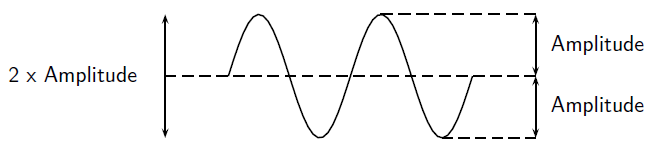
\includegraphics[width=0.8\columnwidth]{col11305.imgs/m38806_PG10C5_006.png} % m38806;PG10C5\_006.png;;;6.0;8.5;
        
      \vspace{2pt}
    \vspace{.1in}
    
    \end{center}

 \end{figure}   

    \addtocounter{footnote}{-0}
    
        \par 
\label{m38806*secfhsst!!!underscore!!!id212}\vspace{.5cm} 
      
      \noindent
      \hspace*{-30pt}
\includegraphics[width=0.5in]{col11305.imgs/pspencil2.png}   \raisebox{25mm}{   
      \begin{mdframed}[linewidth=4, leftmargin=40, rightmargin=40]  
      \begin{exercise}
    \noindent\textbf{Exercise 7.1:  Amplitude of Sea Waves }
        \label{m38806*probfhsst!!!underscore!!!id213}
        \label{m38806*id318469}If the peak of a wave measures \begin{math}2\phantom{\rule{2pt}{0ex}}\mathrm{m}\end{math} above the still water mark in the harbour, what is the amplitude of the wave? \par 
        \vspace{5pt}
        \label{m38806*solfhsst!!!underscore!!!id216}\noindent\textbf{Solution to Exercise } \label{m38806*listfhsst!!!underscore!!!id216}\begin{enumerate}[noitemsep, label=\textbf{Step} \textbf{\arabic*}. ] 
            \leftskip=20pt\rightskip=\leftskip\item  
        \label{m38806*id318492}The definition of the amplitude is the height of a peak above the equilibrium position. The still water mark is the height of the water at equilibrium and the peak is \begin{math}2\phantom{\rule{2pt}{0ex}}\mathrm{m}\end{math} above this, so the amplitude is \begin{math}2\phantom{\rule{2pt}{0ex}}\mathrm{m}\end{math}. \par 
        \end{enumerate}
         

    \end{exercise}
    \end{mdframed}
    }
    \noindent
  
\label{m38806*secfhsst!!!underscore!!!id221}
            \subsubsection{  Investigation : Wavelength }
            \nopagebreak
            
        \label{m38806*id318517}
          
    \setcounter{subfigure}{0}


	\begin{figure}[H] % horizontal\label{m38806*id318520}
    \begin{center}
    \label{m38806*id318520!!!underscore!!!media}\label{m38806*id318520!!!underscore!!!printimage}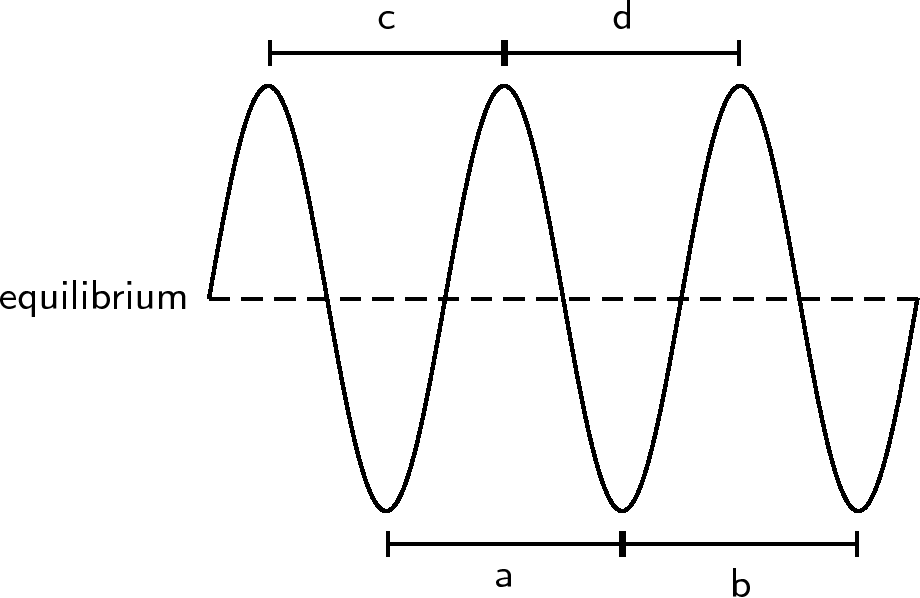
\includegraphics[width=0.5\columnwidth]{col11305.imgs/m38806_PG10C5_007.png} % m38806;PG10C5\_007.png;;;6.0;8.5;
        
      \vspace{2pt}
    \vspace{.1in}
    
    \end{center}

 \end{figure}   

    \addtocounter{footnote}{-0}
    
        \par 
        \label{m38806*id318526}Fill in the table below by measuring the distance between peaks and troughs in the wave above.\par 
        
    % \textbf{m38806*id318530}\par
    
    % how many colspecs?  2
          % name: cnx:colspec
            % colnum: 1
            % colwidth: 10*
            % latex-name: columna
            % colname: 
            % align/tgroup-align/default: //left
            % -------------------------
            % name: cnx:colspec
            % colnum: 2
            % colwidth: 10*
            % latex-name: columnb
            % colname: 
            % align/tgroup-align/default: //left
            % -------------------------
      
    
    \setlength\mytablespace{4\tabcolsep}
    \addtolength\mytablespace{3\arrayrulewidth}
    \setlength\mytablewidth{\linewidth}
        
    
    \setlength\mytableroom{\mytablewidth}
    \addtolength\mytableroom{-\mytablespace}
    
    \setlength\myfixedwidth{0pt}
    \setlength\mystarwidth{\mytableroom}
        \addtolength\mystarwidth{-\myfixedwidth}
        \divide\mystarwidth 20
        
    
      % ----- Begin capturing width of table in LR mode woof
      \settowidth{\mytableboxwidth}{\begin{tabular}[t]{|l|l|}\hline
    % count in rowspan-info-nodeset: 2
    % align/colidx: left,1
    
    % rowcount: '0' | start: 'false' | colidx: '1'
    
        % Formatting a regular cell and recurring on the next sibling
         &
      % align/colidx: left,2
    
    % rowcount: '0' | start: 'false' | colidx: '2'
    
        % Formatting a regular cell and recurring on the next sibling
        Distance(cm)% make-rowspan-placeholders
    % rowspan info: col1 '0' | 'false' | '' || col2 '0' | 'false' | ''
     \tabularnewline\cline{1-1}\cline{2-2}
      %--------------------------------------------------------------------
    % align/colidx: left,1
    
    % rowcount: '0' | start: 'false' | colidx: '1'
    
        % Formatting a regular cell and recurring on the next sibling
        a &
      % align/colidx: left,2
    
    % rowcount: '0' | start: 'false' | colidx: '2'
    
        % Formatting a regular cell and recurring on the next sibling
        % make-rowspan-placeholders
    % rowspan info: col1 '0' | 'false' | '' || col2 '0' | 'false' | ''
     \tabularnewline\cline{1-1}\cline{2-2}
      %--------------------------------------------------------------------
    % align/colidx: left,1
    
    % rowcount: '0' | start: 'false' | colidx: '1'
    
        % Formatting a regular cell and recurring on the next sibling
        b &
      % align/colidx: left,2
    
    % rowcount: '0' | start: 'false' | colidx: '2'
    
        % Formatting a regular cell and recurring on the next sibling
        % make-rowspan-placeholders
    % rowspan info: col1 '0' | 'false' | '' || col2 '0' | 'false' | ''
     \tabularnewline\cline{1-1}\cline{2-2}
      %--------------------------------------------------------------------
    % align/colidx: left,1
    
    % rowcount: '0' | start: 'false' | colidx: '1'
    
        % Formatting a regular cell and recurring on the next sibling
        c &
      % align/colidx: left,2
    
    % rowcount: '0' | start: 'false' | colidx: '2'
    
        % Formatting a regular cell and recurring on the next sibling
        % make-rowspan-placeholders
    % rowspan info: col1 '0' | 'false' | '' || col2 '0' | 'false' | ''
     \tabularnewline\cline{1-1}\cline{2-2}
      %--------------------------------------------------------------------
    % align/colidx: left,1
    
    % rowcount: '0' | start: 'false' | colidx: '1'
    
        % Formatting a regular cell and recurring on the next sibling
        d &
      % align/colidx: left,2
    
    % rowcount: '0' | start: 'false' | colidx: '2'
    
        % Formatting a regular cell and recurring on the next sibling
        % make-rowspan-placeholders
    % rowspan info: col1 '0' | 'false' | '' || col2 '0' | 'false' | ''
     \tabularnewline\cline{1-1}\cline{2-2}
      %--------------------------------------------------------------------
    \end{tabular}} % end mytableboxwidth set
      \addtocounter{footnote}{-0}
      
      % ----- End capturing width of table in LR mode
    
        % ----- LR or paragraph mode: must test
        % ----- Begin capturing height of table
        \settoheight{\mytableboxheight}{\begin{tabular}[t]{|l|l|}\hline
    % count in rowspan-info-nodeset: 2
    % align/colidx: left,1
    
    % rowcount: '0' | start: 'false' | colidx: '1'
    
        % Formatting a regular cell and recurring on the next sibling
         &
      % align/colidx: left,2
    
    % rowcount: '0' | start: 'false' | colidx: '2'
    
        % Formatting a regular cell and recurring on the next sibling
        Distance(cm)% make-rowspan-placeholders
    % rowspan info: col1 '0' | 'false' | '' || col2 '0' | 'false' | ''
     \tabularnewline\cline{1-1}\cline{2-2}
      %--------------------------------------------------------------------
    % align/colidx: left,1
    
    % rowcount: '0' | start: 'false' | colidx: '1'
    
        % Formatting a regular cell and recurring on the next sibling
        a &
      % align/colidx: left,2
    
    % rowcount: '0' | start: 'false' | colidx: '2'
    
        % Formatting a regular cell and recurring on the next sibling
        % make-rowspan-placeholders
    % rowspan info: col1 '0' | 'false' | '' || col2 '0' | 'false' | ''
     \tabularnewline\cline{1-1}\cline{2-2}
      %--------------------------------------------------------------------
    % align/colidx: left,1
    
    % rowcount: '0' | start: 'false' | colidx: '1'
    
        % Formatting a regular cell and recurring on the next sibling
        b &
      % align/colidx: left,2
    
    % rowcount: '0' | start: 'false' | colidx: '2'
    
        % Formatting a regular cell and recurring on the next sibling
        % make-rowspan-placeholders
    % rowspan info: col1 '0' | 'false' | '' || col2 '0' | 'false' | ''
     \tabularnewline\cline{1-1}\cline{2-2}
      %--------------------------------------------------------------------
    % align/colidx: left,1
    
    % rowcount: '0' | start: 'false' | colidx: '1'
    
        % Formatting a regular cell and recurring on the next sibling
        c &
      % align/colidx: left,2
    
    % rowcount: '0' | start: 'false' | colidx: '2'
    
        % Formatting a regular cell and recurring on the next sibling
        % make-rowspan-placeholders
    % rowspan info: col1 '0' | 'false' | '' || col2 '0' | 'false' | ''
     \tabularnewline\cline{1-1}\cline{2-2}
      %--------------------------------------------------------------------
    % align/colidx: left,1
    
    % rowcount: '0' | start: 'false' | colidx: '1'
    
        % Formatting a regular cell and recurring on the next sibling
        d &
      % align/colidx: left,2
    
    % rowcount: '0' | start: 'false' | colidx: '2'
    
        % Formatting a regular cell and recurring on the next sibling
        % make-rowspan-placeholders
    % rowspan info: col1 '0' | 'false' | '' || col2 '0' | 'false' | ''
     \tabularnewline\cline{1-1}\cline{2-2}
      %--------------------------------------------------------------------
    \end{tabular}} % end mytableboxheight set
        \settodepth{\mytableboxdepth}{\begin{tabular}[t]{|l|l|}\hline
    % count in rowspan-info-nodeset: 2
    % align/colidx: left,1
    
    % rowcount: '0' | start: 'false' | colidx: '1'
    
        % Formatting a regular cell and recurring on the next sibling
         &
      % align/colidx: left,2
    
    % rowcount: '0' | start: 'false' | colidx: '2'
    
        % Formatting a regular cell and recurring on the next sibling
        Distance(cm)% make-rowspan-placeholders
    % rowspan info: col1 '0' | 'false' | '' || col2 '0' | 'false' | ''
     \tabularnewline\cline{1-1}\cline{2-2}
      %--------------------------------------------------------------------
    % align/colidx: left,1
    
    % rowcount: '0' | start: 'false' | colidx: '1'
    
        % Formatting a regular cell and recurring on the next sibling
        a &
      % align/colidx: left,2
    
    % rowcount: '0' | start: 'false' | colidx: '2'
    
        % Formatting a regular cell and recurring on the next sibling
        % make-rowspan-placeholders
    % rowspan info: col1 '0' | 'false' | '' || col2 '0' | 'false' | ''
     \tabularnewline\cline{1-1}\cline{2-2}
      %--------------------------------------------------------------------
    % align/colidx: left,1
    
    % rowcount: '0' | start: 'false' | colidx: '1'
    
        % Formatting a regular cell and recurring on the next sibling
        b &
      % align/colidx: left,2
    
    % rowcount: '0' | start: 'false' | colidx: '2'
    
        % Formatting a regular cell and recurring on the next sibling
        % make-rowspan-placeholders
    % rowspan info: col1 '0' | 'false' | '' || col2 '0' | 'false' | ''
     \tabularnewline\cline{1-1}\cline{2-2}
      %--------------------------------------------------------------------
    % align/colidx: left,1
    
    % rowcount: '0' | start: 'false' | colidx: '1'
    
        % Formatting a regular cell and recurring on the next sibling
        c &
      % align/colidx: left,2
    
    % rowcount: '0' | start: 'false' | colidx: '2'
    
        % Formatting a regular cell and recurring on the next sibling
        % make-rowspan-placeholders
    % rowspan info: col1 '0' | 'false' | '' || col2 '0' | 'false' | ''
     \tabularnewline\cline{1-1}\cline{2-2}
      %--------------------------------------------------------------------
    % align/colidx: left,1
    
    % rowcount: '0' | start: 'false' | colidx: '1'
    
        % Formatting a regular cell and recurring on the next sibling
        d &
      % align/colidx: left,2
    
    % rowcount: '0' | start: 'false' | colidx: '2'
    
        % Formatting a regular cell and recurring on the next sibling
        % make-rowspan-placeholders
    % rowspan info: col1 '0' | 'false' | '' || col2 '0' | 'false' | ''
     \tabularnewline\cline{1-1}\cline{2-2}
      %--------------------------------------------------------------------
    \end{tabular}} % end mytableboxdepth set
        \addtolength{\mytableboxheight}{\mytableboxdepth}
        % ----- End capturing height of table
        \addtocounter{footnote}{-0}
        
        \ifthenelse{\mytableboxwidth<\textwidth}{% the table fits in LR mode
          \addtolength{\mytableboxwidth}{-\mytablespace}
          \typeout{textheight: \the\textheight}
          \typeout{mytableboxheight: \the\mytableboxheight}
          \typeout{textwidth: \the\textwidth}
          \typeout{mytableboxwidth: \the\mytableboxwidth}
          \ifthenelse{\mytableboxheight<\textheight}{%
        
    % \begin{table}[H]
    % \\ '' '0'
    
        \begin{center}
      
      \label{m38806*id318530}
      
    \noindent
    \begin{tabular}[t]{|l|l|}\hline
    % count in rowspan-info-nodeset: 2
    % align/colidx: left,1
    
    % rowcount: '0' | start: 'false' | colidx: '1'
    
        % Formatting a regular cell and recurring on the next sibling
         &
      % align/colidx: left,2
    
    % rowcount: '0' | start: 'false' | colidx: '2'
    
        % Formatting a regular cell and recurring on the next sibling
        Distance(cm)% make-rowspan-placeholders
    % rowspan info: col1 '0' | 'false' | '' || col2 '0' | 'false' | ''
     \tabularnewline\cline{1-1}\cline{2-2}
      %--------------------------------------------------------------------
    % align/colidx: left,1
    
    % rowcount: '0' | start: 'false' | colidx: '1'
    
        % Formatting a regular cell and recurring on the next sibling
        a &
      % align/colidx: left,2
    
    % rowcount: '0' | start: 'false' | colidx: '2'
    
        % Formatting a regular cell and recurring on the next sibling
        % make-rowspan-placeholders
    % rowspan info: col1 '0' | 'false' | '' || col2 '0' | 'false' | ''
     \tabularnewline\cline{1-1}\cline{2-2}
      %--------------------------------------------------------------------
    % align/colidx: left,1
    
    % rowcount: '0' | start: 'false' | colidx: '1'
    
        % Formatting a regular cell and recurring on the next sibling
        b &
      % align/colidx: left,2
    
    % rowcount: '0' | start: 'false' | colidx: '2'
    
        % Formatting a regular cell and recurring on the next sibling
        % make-rowspan-placeholders
    % rowspan info: col1 '0' | 'false' | '' || col2 '0' | 'false' | ''
     \tabularnewline\cline{1-1}\cline{2-2}
      %--------------------------------------------------------------------
    % align/colidx: left,1
    
    % rowcount: '0' | start: 'false' | colidx: '1'
    
        % Formatting a regular cell and recurring on the next sibling
        c &
      % align/colidx: left,2
    
    % rowcount: '0' | start: 'false' | colidx: '2'
    
        % Formatting a regular cell and recurring on the next sibling
        % make-rowspan-placeholders
    % rowspan info: col1 '0' | 'false' | '' || col2 '0' | 'false' | ''
     \tabularnewline\cline{1-1}\cline{2-2}
      %--------------------------------------------------------------------
    % align/colidx: left,1
    
    % rowcount: '0' | start: 'false' | colidx: '1'
    
        % Formatting a regular cell and recurring on the next sibling
        d &
      % align/colidx: left,2
    
    % rowcount: '0' | start: 'false' | colidx: '2'
    
        % Formatting a regular cell and recurring on the next sibling
        % make-rowspan-placeholders
    % rowspan info: col1 '0' | 'false' | '' || col2 '0' | 'false' | ''
     \tabularnewline\cline{1-1}\cline{2-2}
      %--------------------------------------------------------------------
    \end{tabular}
      \end{center}
    \begin{center}{\small\bfseries Table 7.2}\end{center}
    %\end{table}
    
    \addtocounter{footnote}{-0}
    
          }{ % else
        
    % \begin{table}[H]
    % \\ '' '0'
    
        \begin{center}
      
      \label{m38806*id318530}
      
    \noindent
    \tabletail{%
        \hline
        \multicolumn{2}{|p{\mytableboxwidth}|}{\raggedleft \small \sl continued on next page}\\
        \hline
      }
      \tablelasttail{}
      \begin{xtabular}[t]{|l|l|}\hline
    % count in rowspan-info-nodeset: 2
    % align/colidx: left,1
    
    % rowcount: '0' | start: 'false' | colidx: '1'
    
        % Formatting a regular cell and recurring on the next sibling
         &
      % align/colidx: left,2
    
    % rowcount: '0' | start: 'false' | colidx: '2'
    
        % Formatting a regular cell and recurring on the next sibling
        Distance(cm)% make-rowspan-placeholders
    % rowspan info: col1 '0' | 'false' | '' || col2 '0' | 'false' | ''
     \tabularnewline\cline{1-1}\cline{2-2}
      %--------------------------------------------------------------------
    % align/colidx: left,1
    
    % rowcount: '0' | start: 'false' | colidx: '1'
    
        % Formatting a regular cell and recurring on the next sibling
        a &
      % align/colidx: left,2
    
    % rowcount: '0' | start: 'false' | colidx: '2'
    
        % Formatting a regular cell and recurring on the next sibling
        % make-rowspan-placeholders
    % rowspan info: col1 '0' | 'false' | '' || col2 '0' | 'false' | ''
     \tabularnewline\cline{1-1}\cline{2-2}
      %--------------------------------------------------------------------
    % align/colidx: left,1
    
    % rowcount: '0' | start: 'false' | colidx: '1'
    
        % Formatting a regular cell and recurring on the next sibling
        b &
      % align/colidx: left,2
    
    % rowcount: '0' | start: 'false' | colidx: '2'
    
        % Formatting a regular cell and recurring on the next sibling
        % make-rowspan-placeholders
    % rowspan info: col1 '0' | 'false' | '' || col2 '0' | 'false' | ''
     \tabularnewline\cline{1-1}\cline{2-2}
      %--------------------------------------------------------------------
    % align/colidx: left,1
    
    % rowcount: '0' | start: 'false' | colidx: '1'
    
        % Formatting a regular cell and recurring on the next sibling
        c &
      % align/colidx: left,2
    
    % rowcount: '0' | start: 'false' | colidx: '2'
    
        % Formatting a regular cell and recurring on the next sibling
        % make-rowspan-placeholders
    % rowspan info: col1 '0' | 'false' | '' || col2 '0' | 'false' | ''
     \tabularnewline\cline{1-1}\cline{2-2}
      %--------------------------------------------------------------------
    % align/colidx: left,1
    
    % rowcount: '0' | start: 'false' | colidx: '1'
    
        % Formatting a regular cell and recurring on the next sibling
        d &
      % align/colidx: left,2
    
    % rowcount: '0' | start: 'false' | colidx: '2'
    
        % Formatting a regular cell and recurring on the next sibling
        % make-rowspan-placeholders
    % rowspan info: col1 '0' | 'false' | '' || col2 '0' | 'false' | ''
     \tabularnewline\cline{1-1}\cline{2-2}
      %--------------------------------------------------------------------
    \end{xtabular}
      \end{center}
    \begin{center}{\small\bfseries Table 7.2}\end{center}
    %\end{table}
    
    \addtocounter{footnote}{-0}
    
          } % 
        }{% else
        % typeset the table in paragraph mode
        % ----- Begin capturing height of table
        \settoheight{\mytableboxheight}{\begin{tabular*}{\mytablewidth}[t]{|p{10\mystarwidth}|p{10\mystarwidth}|}\hline
    % count in rowspan-info-nodeset: 2
    % align/colidx: left,1
    
    % rowcount: '0' | start: 'false' | colidx: '1'
    
        % Formatting a regular cell and recurring on the next sibling
         &
      % align/colidx: left,2
    
    % rowcount: '0' | start: 'false' | colidx: '2'
    
        % Formatting a regular cell and recurring on the next sibling
        Distance(cm)% make-rowspan-placeholders
    % rowspan info: col1 '0' | 'false' | '' || col2 '0' | 'false' | ''
     \tabularnewline\cline{1-1}\cline{2-2}
      %--------------------------------------------------------------------
    % align/colidx: left,1
    
    % rowcount: '0' | start: 'false' | colidx: '1'
    
        % Formatting a regular cell and recurring on the next sibling
        a &
      % align/colidx: left,2
    
    % rowcount: '0' | start: 'false' | colidx: '2'
    
        % Formatting a regular cell and recurring on the next sibling
        % make-rowspan-placeholders
    % rowspan info: col1 '0' | 'false' | '' || col2 '0' | 'false' | ''
     \tabularnewline\cline{1-1}\cline{2-2}
      %--------------------------------------------------------------------
    % align/colidx: left,1
    
    % rowcount: '0' | start: 'false' | colidx: '1'
    
        % Formatting a regular cell and recurring on the next sibling
        b &
      % align/colidx: left,2
    
    % rowcount: '0' | start: 'false' | colidx: '2'
    
        % Formatting a regular cell and recurring on the next sibling
        % make-rowspan-placeholders
    % rowspan info: col1 '0' | 'false' | '' || col2 '0' | 'false' | ''
     \tabularnewline\cline{1-1}\cline{2-2}
      %--------------------------------------------------------------------
    % align/colidx: left,1
    
    % rowcount: '0' | start: 'false' | colidx: '1'
    
        % Formatting a regular cell and recurring on the next sibling
        c &
      % align/colidx: left,2
    
    % rowcount: '0' | start: 'false' | colidx: '2'
    
        % Formatting a regular cell and recurring on the next sibling
        % make-rowspan-placeholders
    % rowspan info: col1 '0' | 'false' | '' || col2 '0' | 'false' | ''
     \tabularnewline\cline{1-1}\cline{2-2}
      %--------------------------------------------------------------------
    % align/colidx: left,1
    
    % rowcount: '0' | start: 'false' | colidx: '1'
    
        % Formatting a regular cell and recurring on the next sibling
        d &
      % align/colidx: left,2
    
    % rowcount: '0' | start: 'false' | colidx: '2'
    
        % Formatting a regular cell and recurring on the next sibling
        % make-rowspan-placeholders
    % rowspan info: col1 '0' | 'false' | '' || col2 '0' | 'false' | ''
     \tabularnewline\cline{1-1}\cline{2-2}
      %--------------------------------------------------------------------
    \end{tabular*}} % end mytableboxheight set
        \settodepth{\mytableboxdepth}{\begin{tabular*}{\mytablewidth}[t]{|p{10\mystarwidth}|p{10\mystarwidth}|}\hline
    % count in rowspan-info-nodeset: 2
    % align/colidx: left,1
    
    % rowcount: '0' | start: 'false' | colidx: '1'
    
        % Formatting a regular cell and recurring on the next sibling
         &
      % align/colidx: left,2
    
    % rowcount: '0' | start: 'false' | colidx: '2'
    
        % Formatting a regular cell and recurring on the next sibling
        Distance(cm)% make-rowspan-placeholders
    % rowspan info: col1 '0' | 'false' | '' || col2 '0' | 'false' | ''
     \tabularnewline\cline{1-1}\cline{2-2}
      %--------------------------------------------------------------------
    % align/colidx: left,1
    
    % rowcount: '0' | start: 'false' | colidx: '1'
    
        % Formatting a regular cell and recurring on the next sibling
        a &
      % align/colidx: left,2
    
    % rowcount: '0' | start: 'false' | colidx: '2'
    
        % Formatting a regular cell and recurring on the next sibling
        % make-rowspan-placeholders
    % rowspan info: col1 '0' | 'false' | '' || col2 '0' | 'false' | ''
     \tabularnewline\cline{1-1}\cline{2-2}
      %--------------------------------------------------------------------
    % align/colidx: left,1
    
    % rowcount: '0' | start: 'false' | colidx: '1'
    
        % Formatting a regular cell and recurring on the next sibling
        b &
      % align/colidx: left,2
    
    % rowcount: '0' | start: 'false' | colidx: '2'
    
        % Formatting a regular cell and recurring on the next sibling
        % make-rowspan-placeholders
    % rowspan info: col1 '0' | 'false' | '' || col2 '0' | 'false' | ''
     \tabularnewline\cline{1-1}\cline{2-2}
      %--------------------------------------------------------------------
    % align/colidx: left,1
    
    % rowcount: '0' | start: 'false' | colidx: '1'
    
        % Formatting a regular cell and recurring on the next sibling
        c &
      % align/colidx: left,2
    
    % rowcount: '0' | start: 'false' | colidx: '2'
    
        % Formatting a regular cell and recurring on the next sibling
        % make-rowspan-placeholders
    % rowspan info: col1 '0' | 'false' | '' || col2 '0' | 'false' | ''
     \tabularnewline\cline{1-1}\cline{2-2}
      %--------------------------------------------------------------------
    % align/colidx: left,1
    
    % rowcount: '0' | start: 'false' | colidx: '1'
    
        % Formatting a regular cell and recurring on the next sibling
        d &
      % align/colidx: left,2
    
    % rowcount: '0' | start: 'false' | colidx: '2'
    
        % Formatting a regular cell and recurring on the next sibling
        % make-rowspan-placeholders
    % rowspan info: col1 '0' | 'false' | '' || col2 '0' | 'false' | ''
     \tabularnewline\cline{1-1}\cline{2-2}
      %--------------------------------------------------------------------
    \end{tabular*}} % end mytableboxdepth set
        \addtolength{\mytableboxheight}{\mytableboxdepth}
        % ----- End capturing height of table
        \typeout{textheight: \the\textheight}
        \typeout{mytableboxheight: \the\mytableboxheight}
        \typeout{table too wide, outputting in para mode}
        
    % \begin{table}[H]
    % \\ '' '0'
    
        \begin{center}
      
      \label{m38806*id318530}
      
    \noindent
    \tabletail{%
        \hline
        \multicolumn{2}{|p{\mytableroom}|}{\raggedleft \small \sl continued on next page}\\
        \hline
      }
      \tablelasttail{}
      \begin{xtabular*}{\mytablewidth}[t]{|p{10\mystarwidth}|p{10\mystarwidth}|}\hline
    % count in rowspan-info-nodeset: 2
    % align/colidx: left,1
    
    % rowcount: '0' | start: 'false' | colidx: '1'
    
        % Formatting a regular cell and recurring on the next sibling
         &
      % align/colidx: left,2
    
    % rowcount: '0' | start: 'false' | colidx: '2'
    
        % Formatting a regular cell and recurring on the next sibling
        Distance(cm)% make-rowspan-placeholders
    % rowspan info: col1 '0' | 'false' | '' || col2 '0' | 'false' | ''
     \tabularnewline\cline{1-1}\cline{2-2}
      %--------------------------------------------------------------------
    % align/colidx: left,1
    
    % rowcount: '0' | start: 'false' | colidx: '1'
    
        % Formatting a regular cell and recurring on the next sibling
        a &
      % align/colidx: left,2
    
    % rowcount: '0' | start: 'false' | colidx: '2'
    
        % Formatting a regular cell and recurring on the next sibling
        % make-rowspan-placeholders
    % rowspan info: col1 '0' | 'false' | '' || col2 '0' | 'false' | ''
     \tabularnewline\cline{1-1}\cline{2-2}
      %--------------------------------------------------------------------
    % align/colidx: left,1
    
    % rowcount: '0' | start: 'false' | colidx: '1'
    
        % Formatting a regular cell and recurring on the next sibling
        b &
      % align/colidx: left,2
    
    % rowcount: '0' | start: 'false' | colidx: '2'
    
        % Formatting a regular cell and recurring on the next sibling
        % make-rowspan-placeholders
    % rowspan info: col1 '0' | 'false' | '' || col2 '0' | 'false' | ''
     \tabularnewline\cline{1-1}\cline{2-2}
      %--------------------------------------------------------------------
    % align/colidx: left,1
    
    % rowcount: '0' | start: 'false' | colidx: '1'
    
        % Formatting a regular cell and recurring on the next sibling
        c &
      % align/colidx: left,2
    
    % rowcount: '0' | start: 'false' | colidx: '2'
    
        % Formatting a regular cell and recurring on the next sibling
        % make-rowspan-placeholders
    % rowspan info: col1 '0' | 'false' | '' || col2 '0' | 'false' | ''
     \tabularnewline\cline{1-1}\cline{2-2}
      %--------------------------------------------------------------------
    % align/colidx: left,1
    
    % rowcount: '0' | start: 'false' | colidx: '1'
    
        % Formatting a regular cell and recurring on the next sibling
        d &
      % align/colidx: left,2
    
    % rowcount: '0' | start: 'false' | colidx: '2'
    
        % Formatting a regular cell and recurring on the next sibling
        % make-rowspan-placeholders
    % rowspan info: col1 '0' | 'false' | '' || col2 '0' | 'false' | ''
     \tabularnewline\cline{1-1}\cline{2-2}
      %--------------------------------------------------------------------
    \end{xtabular*}
      \end{center}
    \begin{center}{\small\bfseries Table 7.2}\end{center}
    %\end{table}
    
    \addtocounter{footnote}{-0}
    
        }% ending lr/para test clause
      
    \par
  
        
        \label{m38806*id318631}\begin{enumerate}[noitemsep, label=\textbf{\arabic*}. ] 
            \label{m38806*uid15}\item What can you say about your results?
\label{m38806*uid16}\item Are the distances between peaks equal?
\label{m38806*uid17}\item Are the distances between troughs equal?
\label{m38806*uid18}\item Is the distance between peaks equal to the distance between troughs?
\end{enumerate}
        
        

        \label{m38806*id318690}As we have seen in the activity on wavelength, the distance between two \textsl{adjacent} peaks is the same no matter which two adjacent peaks you choose. There is a fixed distance between the peaks. Similarly, we have seen that there is a fixed distance between the troughs, no matter which two troughs you look at. More importantly, the distance between two adjacent peaks is the same as the distance between two adjacent troughs. This distance is called the \textsl{wavelength} of the wave.\par 
        \label{m38806*id318708}The symbol for the wavelength is \begin{math}\lambda \end{math} (the Greek letter \textsl{lambda}) and wavelength is measured in metres (\begin{math}\mathrm{m}\end{math}).\par 
        \label{m38806*id318725}
    \setcounter{subfigure}{0}


	\begin{figure}[H] % horizontal\label{m38806*id318728}
    \begin{center}
    \label{m38806*id318728!!!underscore!!!media}\label{m38806*id318728!!!underscore!!!printimage}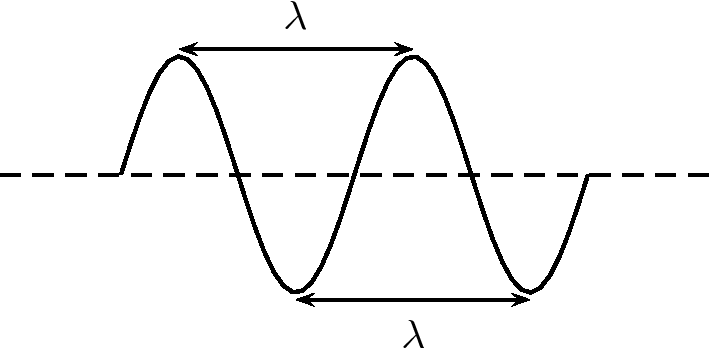
\includegraphics[width=0.5\columnwidth]{col11305.imgs/m38806_PG10C5_008.png} % m38806;PG10C5\_008.png;;;6.0;8.5;
        
      \vspace{2pt}
    \vspace{.1in}
    
    \end{center}

 \end{figure}   

    \addtocounter{footnote}{-0}
    
        \par 
\label{m38806*secfhsst!!!underscore!!!id280}\vspace{.5cm} 
      
      \noindent
      \hspace*{-30pt}
\includegraphics[width=0.5in]{col11305.imgs/pspencil2.png}   \raisebox{25mm}{   
      \begin{mdframed}[linewidth=4, leftmargin=40, rightmargin=40]  
      \begin{exercise}
    \noindent\textbf{Exercise 7.2:  Wavelength }
        \label{m38806*probfhsst!!!underscore!!!id281}
        \label{m38806*id318746}The total distance between \begin{math}4\end{math} consecutive peaks of a transverse wave is \begin{math}6\phantom{\rule{2pt}{0ex}}\mathrm{m}\end{math}. What is the wavelength of the wave? \par 
        \vspace{5pt}
        \label{m38806*solfhsst!!!underscore!!!id284}\noindent\textbf{Solution to Exercise } \label{m38806*listfhsst!!!underscore!!!id284}\begin{enumerate}[noitemsep, label=\textbf{Step} \textbf{\arabic*}. ] 
            \leftskip=20pt\rightskip=\leftskip\item  
        \label{m38806*id318770}
          
    \setcounter{subfigure}{0}


	\begin{figure}[H] % horizontal\label{m38806*id318773}
    \begin{center}
    \label{m38806*id318773!!!underscore!!!media}\label{m38806*id318773!!!underscore!!!printimage}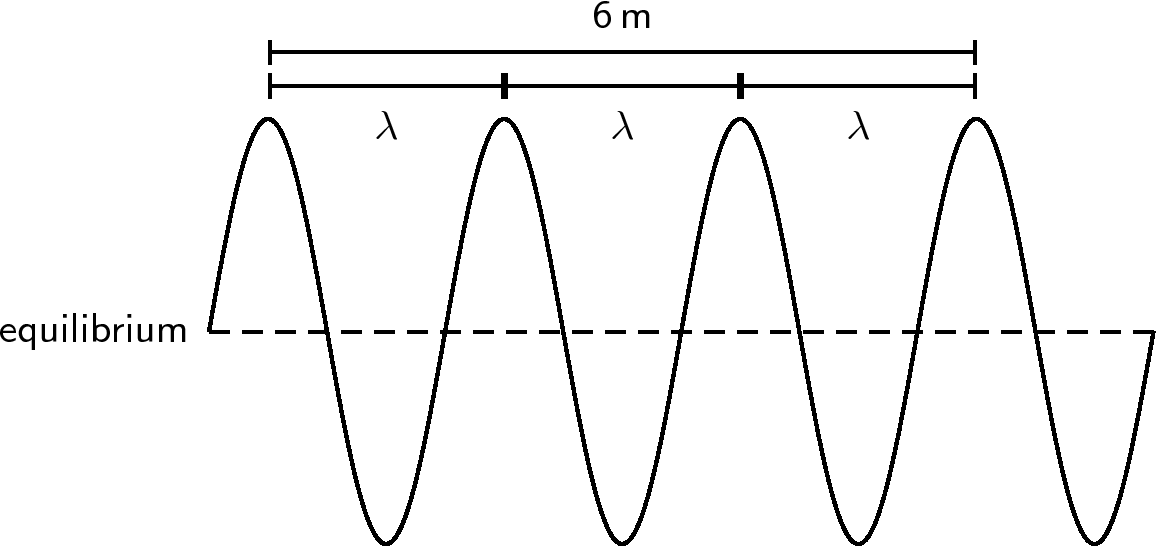
\includegraphics{col11305.imgs/m38806_PG10C5_009.png} % ;PG10C5\_009.png;;;6.0;8.5;
        
      \vspace{2pt}
    \vspace{.1in}
    
    \end{center}

 \end{figure}   

    \addtocounter{footnote}{-0}
    
        \par 
        \item  
        \label{m38806*id318783}From the sketch we see that 4 consecutive peaks is equivalent to 3 wavelengths.\par 
        \item  
        \label{m38806*id318791}Therefore, the wavelength of the wave is:\par 
        \label{m38806*id318795}\nopagebreak\noindent{}
          \settowidth{\mymathboxwidth}{\begin{equation}
    \begin{array}{ccc}\hfill 3\lambda & =& 6\phantom{\rule{0.166667em}{0ex}}\mathrm{m}\hfill \\ \hfill \lambda & =& \frac{6\phantom{\rule{0.166667em}{0ex}}\mathrm{m}}{3}\hfill \\ & =& 2\phantom{\rule{0.166667em}{0ex}}\mathrm{m}\hfill \end{array}\tag{7.1}
      \end{equation}
    }
    \typeout{Columnwidth = \the\columnwidth}\typeout{math as usual width = \the\mymathboxwidth}
    \ifthenelse{\lengthtest{\mymathboxwidth < \columnwidth}}{% if the math fits, do it again, for real
    \begin{equation}
    \begin{array}{ccc}\hfill 3\lambda & =& 6\phantom{\rule{0.166667em}{0ex}}\mathrm{m}\hfill \\ \hfill \lambda & =& \frac{6\phantom{\rule{0.166667em}{0ex}}\mathrm{m}}{3}\hfill \\ & =& 2\phantom{\rule{0.166667em}{0ex}}\mathrm{m}\hfill \end{array}\tag{7.1}
      \end{equation}
    }{% else, if it doesn't fit
    \setlength{\mymathboxwidth}{\columnwidth}
      \addtolength{\mymathboxwidth}{-48pt}
    \par\vspace{12pt}\noindent\begin{minipage}{\columnwidth}
    \parbox[t]{\mymathboxwidth}{\large\begin{math}
    3\lambda =6\phantom{\rule{0.166667em}{0ex}}\mathrm{m}\lambda =\frac{6\phantom{\rule{0.166667em}{0ex}}\mathrm{m}}{3}=2\phantom{\rule{0.166667em}{0ex}}\mathrm{m}\end{math}}\hfill
    \parbox[t]{48pt}{\raggedleft 
    (7.1)}
    \end{minipage}\vspace{12pt}\par
    }% end of conditional for this bit of math
    \typeout{math as usual width = \the\mymathboxwidth}
    
        
        
        \end{enumerate}
         

    \end{exercise}
    \end{mdframed}
    }
    \noindent
  
      
      \label{m38806*uid19}
            \subsection{ Points in Phase}
            \nopagebreak
            
        
\label{m38806*secfhsst!!!underscore!!!id359}
            \subsubsection{  Investigation : Points in Phase }
            \nopagebreak
            
        \label{m38806*id318912}Fill in the table by measuring the distance between the indicated points.\par 
        \label{m38806*id318918}
          
    \setcounter{subfigure}{0}


	\begin{figure}[H] % horizontal\label{m38806*id318921}
    \begin{center}
    \label{m38806*id318921!!!underscore!!!media}\label{m38806*id318921!!!underscore!!!printimage}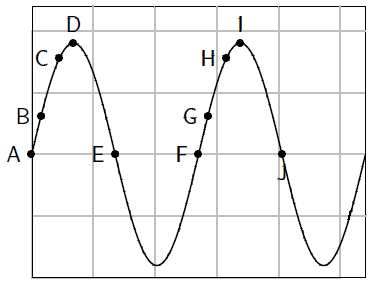
\includegraphics[width=0.4\columnwidth]{col11305.imgs/m38806_PG10C5_010.png} % m38806;PG10C5\_010.png;;;6.0;8.5;
        
      \vspace{2pt}
    \vspace{.1in}
    
    \end{center}

 \end{figure}   

    \addtocounter{footnote}{-0}
    
        \par 
        
    % \textbf{m38806*id318927}\par
    
    % how many colspecs?  2
          % name: cnx:colspec
            % colnum: 1
            % colwidth: 10*
            % latex-name: columna
            % colname: 
            % align/tgroup-align/default: //left
            % -------------------------
            % name: cnx:colspec
            % colnum: 2
            % colwidth: 10*
            % latex-name: columnb
            % colname: 
            % align/tgroup-align/default: //left
            % -------------------------
      
    
    \setlength\mytablespace{4\tabcolsep}
    \addtolength\mytablespace{3\arrayrulewidth}
    \setlength\mytablewidth{\linewidth}
        
    
    \setlength\mytableroom{\mytablewidth}
    \addtolength\mytableroom{-\mytablespace}
    
    \setlength\myfixedwidth{0pt}
    \setlength\mystarwidth{\mytableroom}
        \addtolength\mystarwidth{-\myfixedwidth}
        \divide\mystarwidth 20
        
    
      % ----- Begin capturing width of table in LR mode woof
      \settowidth{\mytableboxwidth}{\begin{tabular}[t]{|l|l|}\hline
    % count in rowspan-info-nodeset: 2
    % align/colidx: left,1
    
    % rowcount: '0' | start: 'false' | colidx: '1'
    
        % Formatting a regular cell and recurring on the next sibling
        
                  \textbf{Points}
                 &
      % align/colidx: left,2
    
    % rowcount: '0' | start: 'false' | colidx: '2'
    
        % Formatting a regular cell and recurring on the next sibling
        
                  \textbf{Distance (cm)}
                % make-rowspan-placeholders
    % rowspan info: col1 '0' | 'false' | '' || col2 '0' | 'false' | ''
     \tabularnewline\cline{1-1}\cline{2-2}
      %--------------------------------------------------------------------
    % align/colidx: left,1
    
    % rowcount: '0' | start: 'false' | colidx: '1'
    
        % Formatting a regular cell and recurring on the next sibling
        A to F &
      % align/colidx: left,2
    
    % rowcount: '0' | start: 'false' | colidx: '2'
    
        % Formatting a regular cell and recurring on the next sibling
        % make-rowspan-placeholders
    % rowspan info: col1 '0' | 'false' | '' || col2 '0' | 'false' | ''
     \tabularnewline\cline{1-1}\cline{2-2}
      %--------------------------------------------------------------------
    % align/colidx: left,1
    
    % rowcount: '0' | start: 'false' | colidx: '1'
    
        % Formatting a regular cell and recurring on the next sibling
        B to G &
      % align/colidx: left,2
    
    % rowcount: '0' | start: 'false' | colidx: '2'
    
        % Formatting a regular cell and recurring on the next sibling
        % make-rowspan-placeholders
    % rowspan info: col1 '0' | 'false' | '' || col2 '0' | 'false' | ''
     \tabularnewline\cline{1-1}\cline{2-2}
      %--------------------------------------------------------------------
    % align/colidx: left,1
    
    % rowcount: '0' | start: 'false' | colidx: '1'
    
        % Formatting a regular cell and recurring on the next sibling
        C to H &
      % align/colidx: left,2
    
    % rowcount: '0' | start: 'false' | colidx: '2'
    
        % Formatting a regular cell and recurring on the next sibling
        % make-rowspan-placeholders
    % rowspan info: col1 '0' | 'false' | '' || col2 '0' | 'false' | ''
     \tabularnewline\cline{1-1}\cline{2-2}
      %--------------------------------------------------------------------
    % align/colidx: left,1
    
    % rowcount: '0' | start: 'false' | colidx: '1'
    
        % Formatting a regular cell and recurring on the next sibling
        D to I &
      % align/colidx: left,2
    
    % rowcount: '0' | start: 'false' | colidx: '2'
    
        % Formatting a regular cell and recurring on the next sibling
        % make-rowspan-placeholders
    % rowspan info: col1 '0' | 'false' | '' || col2 '0' | 'false' | ''
     \tabularnewline\cline{1-1}\cline{2-2}
      %--------------------------------------------------------------------
    % align/colidx: left,1
    
    % rowcount: '0' | start: 'false' | colidx: '1'
    
        % Formatting a regular cell and recurring on the next sibling
        E to J &
      % align/colidx: left,2
    
    % rowcount: '0' | start: 'false' | colidx: '2'
    
        % Formatting a regular cell and recurring on the next sibling
        % make-rowspan-placeholders
    % rowspan info: col1 '0' | 'false' | '' || col2 '0' | 'false' | ''
     \tabularnewline\cline{1-1}\cline{2-2}
      %--------------------------------------------------------------------
    \end{tabular}} % end mytableboxwidth set
      \addtocounter{footnote}{-0}
      
      % ----- End capturing width of table in LR mode
    
        % ----- LR or paragraph mode: must test
        % ----- Begin capturing height of table
        \settoheight{\mytableboxheight}{\begin{tabular}[t]{|l|l|}\hline
    % count in rowspan-info-nodeset: 2
    % align/colidx: left,1
    
    % rowcount: '0' | start: 'false' | colidx: '1'
    
        % Formatting a regular cell and recurring on the next sibling
        
                  \textbf{Points}
                 &
      % align/colidx: left,2
    
    % rowcount: '0' | start: 'false' | colidx: '2'
    
        % Formatting a regular cell and recurring on the next sibling
        
                  \textbf{Distance (cm)}
                % make-rowspan-placeholders
    % rowspan info: col1 '0' | 'false' | '' || col2 '0' | 'false' | ''
     \tabularnewline\cline{1-1}\cline{2-2}
      %--------------------------------------------------------------------
    % align/colidx: left,1
    
    % rowcount: '0' | start: 'false' | colidx: '1'
    
        % Formatting a regular cell and recurring on the next sibling
        A to F &
      % align/colidx: left,2
    
    % rowcount: '0' | start: 'false' | colidx: '2'
    
        % Formatting a regular cell and recurring on the next sibling
        % make-rowspan-placeholders
    % rowspan info: col1 '0' | 'false' | '' || col2 '0' | 'false' | ''
     \tabularnewline\cline{1-1}\cline{2-2}
      %--------------------------------------------------------------------
    % align/colidx: left,1
    
    % rowcount: '0' | start: 'false' | colidx: '1'
    
        % Formatting a regular cell and recurring on the next sibling
        B to G &
      % align/colidx: left,2
    
    % rowcount: '0' | start: 'false' | colidx: '2'
    
        % Formatting a regular cell and recurring on the next sibling
        % make-rowspan-placeholders
    % rowspan info: col1 '0' | 'false' | '' || col2 '0' | 'false' | ''
     \tabularnewline\cline{1-1}\cline{2-2}
      %--------------------------------------------------------------------
    % align/colidx: left,1
    
    % rowcount: '0' | start: 'false' | colidx: '1'
    
        % Formatting a regular cell and recurring on the next sibling
        C to H &
      % align/colidx: left,2
    
    % rowcount: '0' | start: 'false' | colidx: '2'
    
        % Formatting a regular cell and recurring on the next sibling
        % make-rowspan-placeholders
    % rowspan info: col1 '0' | 'false' | '' || col2 '0' | 'false' | ''
     \tabularnewline\cline{1-1}\cline{2-2}
      %--------------------------------------------------------------------
    % align/colidx: left,1
    
    % rowcount: '0' | start: 'false' | colidx: '1'
    
        % Formatting a regular cell and recurring on the next sibling
        D to I &
      % align/colidx: left,2
    
    % rowcount: '0' | start: 'false' | colidx: '2'
    
        % Formatting a regular cell and recurring on the next sibling
        % make-rowspan-placeholders
    % rowspan info: col1 '0' | 'false' | '' || col2 '0' | 'false' | ''
     \tabularnewline\cline{1-1}\cline{2-2}
      %--------------------------------------------------------------------
    % align/colidx: left,1
    
    % rowcount: '0' | start: 'false' | colidx: '1'
    
        % Formatting a regular cell and recurring on the next sibling
        E to J &
      % align/colidx: left,2
    
    % rowcount: '0' | start: 'false' | colidx: '2'
    
        % Formatting a regular cell and recurring on the next sibling
        % make-rowspan-placeholders
    % rowspan info: col1 '0' | 'false' | '' || col2 '0' | 'false' | ''
     \tabularnewline\cline{1-1}\cline{2-2}
      %--------------------------------------------------------------------
    \end{tabular}} % end mytableboxheight set
        \settodepth{\mytableboxdepth}{\begin{tabular}[t]{|l|l|}\hline
    % count in rowspan-info-nodeset: 2
    % align/colidx: left,1
    
    % rowcount: '0' | start: 'false' | colidx: '1'
    
        % Formatting a regular cell and recurring on the next sibling
        
                  \textbf{Points}
                 &
      % align/colidx: left,2
    
    % rowcount: '0' | start: 'false' | colidx: '2'
    
        % Formatting a regular cell and recurring on the next sibling
        
                  \textbf{Distance (cm)}
                % make-rowspan-placeholders
    % rowspan info: col1 '0' | 'false' | '' || col2 '0' | 'false' | ''
     \tabularnewline\cline{1-1}\cline{2-2}
      %--------------------------------------------------------------------
    % align/colidx: left,1
    
    % rowcount: '0' | start: 'false' | colidx: '1'
    
        % Formatting a regular cell and recurring on the next sibling
        A to F &
      % align/colidx: left,2
    
    % rowcount: '0' | start: 'false' | colidx: '2'
    
        % Formatting a regular cell and recurring on the next sibling
        % make-rowspan-placeholders
    % rowspan info: col1 '0' | 'false' | '' || col2 '0' | 'false' | ''
     \tabularnewline\cline{1-1}\cline{2-2}
      %--------------------------------------------------------------------
    % align/colidx: left,1
    
    % rowcount: '0' | start: 'false' | colidx: '1'
    
        % Formatting a regular cell and recurring on the next sibling
        B to G &
      % align/colidx: left,2
    
    % rowcount: '0' | start: 'false' | colidx: '2'
    
        % Formatting a regular cell and recurring on the next sibling
        % make-rowspan-placeholders
    % rowspan info: col1 '0' | 'false' | '' || col2 '0' | 'false' | ''
     \tabularnewline\cline{1-1}\cline{2-2}
      %--------------------------------------------------------------------
    % align/colidx: left,1
    
    % rowcount: '0' | start: 'false' | colidx: '1'
    
        % Formatting a regular cell and recurring on the next sibling
        C to H &
      % align/colidx: left,2
    
    % rowcount: '0' | start: 'false' | colidx: '2'
    
        % Formatting a regular cell and recurring on the next sibling
        % make-rowspan-placeholders
    % rowspan info: col1 '0' | 'false' | '' || col2 '0' | 'false' | ''
     \tabularnewline\cline{1-1}\cline{2-2}
      %--------------------------------------------------------------------
    % align/colidx: left,1
    
    % rowcount: '0' | start: 'false' | colidx: '1'
    
        % Formatting a regular cell and recurring on the next sibling
        D to I &
      % align/colidx: left,2
    
    % rowcount: '0' | start: 'false' | colidx: '2'
    
        % Formatting a regular cell and recurring on the next sibling
        % make-rowspan-placeholders
    % rowspan info: col1 '0' | 'false' | '' || col2 '0' | 'false' | ''
     \tabularnewline\cline{1-1}\cline{2-2}
      %--------------------------------------------------------------------
    % align/colidx: left,1
    
    % rowcount: '0' | start: 'false' | colidx: '1'
    
        % Formatting a regular cell and recurring on the next sibling
        E to J &
      % align/colidx: left,2
    
    % rowcount: '0' | start: 'false' | colidx: '2'
    
        % Formatting a regular cell and recurring on the next sibling
        % make-rowspan-placeholders
    % rowspan info: col1 '0' | 'false' | '' || col2 '0' | 'false' | ''
     \tabularnewline\cline{1-1}\cline{2-2}
      %--------------------------------------------------------------------
    \end{tabular}} % end mytableboxdepth set
        \addtolength{\mytableboxheight}{\mytableboxdepth}
        % ----- End capturing height of table
        \addtocounter{footnote}{-0}
        
        \ifthenelse{\mytableboxwidth<\textwidth}{% the table fits in LR mode
          \addtolength{\mytableboxwidth}{-\mytablespace}
          \typeout{textheight: \the\textheight}
          \typeout{mytableboxheight: \the\mytableboxheight}
          \typeout{textwidth: \the\textwidth}
          \typeout{mytableboxwidth: \the\mytableboxwidth}
          \ifthenelse{\mytableboxheight<\textheight}{%
        
    % \begin{table}[H]
    % \\ '' '0'
    
        \begin{center}
      
      \label{m38806*id318927}
      
    \noindent
    \begin{tabular}[t]{|l|l|}\hline
    % count in rowspan-info-nodeset: 2
    % align/colidx: left,1
    
    % rowcount: '0' | start: 'false' | colidx: '1'
    
        % Formatting a regular cell and recurring on the next sibling
        
                  \textbf{Points}
                 &
      % align/colidx: left,2
    
    % rowcount: '0' | start: 'false' | colidx: '2'
    
        % Formatting a regular cell and recurring on the next sibling
        
                  \textbf{Distance (cm)}
                % make-rowspan-placeholders
    % rowspan info: col1 '0' | 'false' | '' || col2 '0' | 'false' | ''
     \tabularnewline\cline{1-1}\cline{2-2}
      %--------------------------------------------------------------------
    % align/colidx: left,1
    
    % rowcount: '0' | start: 'false' | colidx: '1'
    
        % Formatting a regular cell and recurring on the next sibling
        A to F &
      % align/colidx: left,2
    
    % rowcount: '0' | start: 'false' | colidx: '2'
    
        % Formatting a regular cell and recurring on the next sibling
        % make-rowspan-placeholders
    % rowspan info: col1 '0' | 'false' | '' || col2 '0' | 'false' | ''
     \tabularnewline\cline{1-1}\cline{2-2}
      %--------------------------------------------------------------------
    % align/colidx: left,1
    
    % rowcount: '0' | start: 'false' | colidx: '1'
    
        % Formatting a regular cell and recurring on the next sibling
        B to G &
      % align/colidx: left,2
    
    % rowcount: '0' | start: 'false' | colidx: '2'
    
        % Formatting a regular cell and recurring on the next sibling
        % make-rowspan-placeholders
    % rowspan info: col1 '0' | 'false' | '' || col2 '0' | 'false' | ''
     \tabularnewline\cline{1-1}\cline{2-2}
      %--------------------------------------------------------------------
    % align/colidx: left,1
    
    % rowcount: '0' | start: 'false' | colidx: '1'
    
        % Formatting a regular cell and recurring on the next sibling
        C to H &
      % align/colidx: left,2
    
    % rowcount: '0' | start: 'false' | colidx: '2'
    
        % Formatting a regular cell and recurring on the next sibling
        % make-rowspan-placeholders
    % rowspan info: col1 '0' | 'false' | '' || col2 '0' | 'false' | ''
     \tabularnewline\cline{1-1}\cline{2-2}
      %--------------------------------------------------------------------
    % align/colidx: left,1
    
    % rowcount: '0' | start: 'false' | colidx: '1'
    
        % Formatting a regular cell and recurring on the next sibling
        D to I &
      % align/colidx: left,2
    
    % rowcount: '0' | start: 'false' | colidx: '2'
    
        % Formatting a regular cell and recurring on the next sibling
        % make-rowspan-placeholders
    % rowspan info: col1 '0' | 'false' | '' || col2 '0' | 'false' | ''
     \tabularnewline\cline{1-1}\cline{2-2}
      %--------------------------------------------------------------------
    % align/colidx: left,1
    
    % rowcount: '0' | start: 'false' | colidx: '1'
    
        % Formatting a regular cell and recurring on the next sibling
        E to J &
      % align/colidx: left,2
    
    % rowcount: '0' | start: 'false' | colidx: '2'
    
        % Formatting a regular cell and recurring on the next sibling
        % make-rowspan-placeholders
    % rowspan info: col1 '0' | 'false' | '' || col2 '0' | 'false' | ''
     \tabularnewline\cline{1-1}\cline{2-2}
      %--------------------------------------------------------------------
    \end{tabular}
      \end{center}
    \begin{center}{\small\bfseries Table 7.3}\end{center}
    %\end{table}
    
    \addtocounter{footnote}{-0}
    
          }{ % else
        
    % \begin{table}[H]
    % \\ '' '0'
    
        \begin{center}
      
      \label{m38806*id318927}
      
    \noindent
    \tabletail{%
        \hline
        \multicolumn{2}{|p{\mytableboxwidth}|}{\raggedleft \small \sl continued on next page}\\
        \hline
      }
      \tablelasttail{}
      \begin{xtabular}[t]{|l|l|}\hline
    % count in rowspan-info-nodeset: 2
    % align/colidx: left,1
    
    % rowcount: '0' | start: 'false' | colidx: '1'
    
        % Formatting a regular cell and recurring on the next sibling
        
                  \textbf{Points}
                 &
      % align/colidx: left,2
    
    % rowcount: '0' | start: 'false' | colidx: '2'
    
        % Formatting a regular cell and recurring on the next sibling
        
                  \textbf{Distance (cm)}
                % make-rowspan-placeholders
    % rowspan info: col1 '0' | 'false' | '' || col2 '0' | 'false' | ''
     \tabularnewline\cline{1-1}\cline{2-2}
      %--------------------------------------------------------------------
    % align/colidx: left,1
    
    % rowcount: '0' | start: 'false' | colidx: '1'
    
        % Formatting a regular cell and recurring on the next sibling
        A to F &
      % align/colidx: left,2
    
    % rowcount: '0' | start: 'false' | colidx: '2'
    
        % Formatting a regular cell and recurring on the next sibling
        % make-rowspan-placeholders
    % rowspan info: col1 '0' | 'false' | '' || col2 '0' | 'false' | ''
     \tabularnewline\cline{1-1}\cline{2-2}
      %--------------------------------------------------------------------
    % align/colidx: left,1
    
    % rowcount: '0' | start: 'false' | colidx: '1'
    
        % Formatting a regular cell and recurring on the next sibling
        B to G &
      % align/colidx: left,2
    
    % rowcount: '0' | start: 'false' | colidx: '2'
    
        % Formatting a regular cell and recurring on the next sibling
        % make-rowspan-placeholders
    % rowspan info: col1 '0' | 'false' | '' || col2 '0' | 'false' | ''
     \tabularnewline\cline{1-1}\cline{2-2}
      %--------------------------------------------------------------------
    % align/colidx: left,1
    
    % rowcount: '0' | start: 'false' | colidx: '1'
    
        % Formatting a regular cell and recurring on the next sibling
        C to H &
      % align/colidx: left,2
    
    % rowcount: '0' | start: 'false' | colidx: '2'
    
        % Formatting a regular cell and recurring on the next sibling
        % make-rowspan-placeholders
    % rowspan info: col1 '0' | 'false' | '' || col2 '0' | 'false' | ''
     \tabularnewline\cline{1-1}\cline{2-2}
      %--------------------------------------------------------------------
    % align/colidx: left,1
    
    % rowcount: '0' | start: 'false' | colidx: '1'
    
        % Formatting a regular cell and recurring on the next sibling
        D to I &
      % align/colidx: left,2
    
    % rowcount: '0' | start: 'false' | colidx: '2'
    
        % Formatting a regular cell and recurring on the next sibling
        % make-rowspan-placeholders
    % rowspan info: col1 '0' | 'false' | '' || col2 '0' | 'false' | ''
     \tabularnewline\cline{1-1}\cline{2-2}
      %--------------------------------------------------------------------
    % align/colidx: left,1
    
    % rowcount: '0' | start: 'false' | colidx: '1'
    
        % Formatting a regular cell and recurring on the next sibling
        E to J &
      % align/colidx: left,2
    
    % rowcount: '0' | start: 'false' | colidx: '2'
    
        % Formatting a regular cell and recurring on the next sibling
        % make-rowspan-placeholders
    % rowspan info: col1 '0' | 'false' | '' || col2 '0' | 'false' | ''
     \tabularnewline\cline{1-1}\cline{2-2}
      %--------------------------------------------------------------------
    \end{xtabular}
      \end{center}
    \begin{center}{\small\bfseries Table 7.3}\end{center}
    %\end{table}
    
    \addtocounter{footnote}{-0}
    
          } % 
        }{% else
        % typeset the table in paragraph mode
        % ----- Begin capturing height of table
        \settoheight{\mytableboxheight}{\begin{tabular*}{\mytablewidth}[t]{|p{10\mystarwidth}|p{10\mystarwidth}|}\hline
    % count in rowspan-info-nodeset: 2
    % align/colidx: left,1
    
    % rowcount: '0' | start: 'false' | colidx: '1'
    
        % Formatting a regular cell and recurring on the next sibling
        
                  \textbf{Points}
                 &
      % align/colidx: left,2
    
    % rowcount: '0' | start: 'false' | colidx: '2'
    
        % Formatting a regular cell and recurring on the next sibling
        
                  \textbf{Distance (cm)}
                % make-rowspan-placeholders
    % rowspan info: col1 '0' | 'false' | '' || col2 '0' | 'false' | ''
     \tabularnewline\cline{1-1}\cline{2-2}
      %--------------------------------------------------------------------
    % align/colidx: left,1
    
    % rowcount: '0' | start: 'false' | colidx: '1'
    
        % Formatting a regular cell and recurring on the next sibling
        A to F &
      % align/colidx: left,2
    
    % rowcount: '0' | start: 'false' | colidx: '2'
    
        % Formatting a regular cell and recurring on the next sibling
        % make-rowspan-placeholders
    % rowspan info: col1 '0' | 'false' | '' || col2 '0' | 'false' | ''
     \tabularnewline\cline{1-1}\cline{2-2}
      %--------------------------------------------------------------------
    % align/colidx: left,1
    
    % rowcount: '0' | start: 'false' | colidx: '1'
    
        % Formatting a regular cell and recurring on the next sibling
        B to G &
      % align/colidx: left,2
    
    % rowcount: '0' | start: 'false' | colidx: '2'
    
        % Formatting a regular cell and recurring on the next sibling
        % make-rowspan-placeholders
    % rowspan info: col1 '0' | 'false' | '' || col2 '0' | 'false' | ''
     \tabularnewline\cline{1-1}\cline{2-2}
      %--------------------------------------------------------------------
    % align/colidx: left,1
    
    % rowcount: '0' | start: 'false' | colidx: '1'
    
        % Formatting a regular cell and recurring on the next sibling
        C to H &
      % align/colidx: left,2
    
    % rowcount: '0' | start: 'false' | colidx: '2'
    
        % Formatting a regular cell and recurring on the next sibling
        % make-rowspan-placeholders
    % rowspan info: col1 '0' | 'false' | '' || col2 '0' | 'false' | ''
     \tabularnewline\cline{1-1}\cline{2-2}
      %--------------------------------------------------------------------
    % align/colidx: left,1
    
    % rowcount: '0' | start: 'false' | colidx: '1'
    
        % Formatting a regular cell and recurring on the next sibling
        D to I &
      % align/colidx: left,2
    
    % rowcount: '0' | start: 'false' | colidx: '2'
    
        % Formatting a regular cell and recurring on the next sibling
        % make-rowspan-placeholders
    % rowspan info: col1 '0' | 'false' | '' || col2 '0' | 'false' | ''
     \tabularnewline\cline{1-1}\cline{2-2}
      %--------------------------------------------------------------------
    % align/colidx: left,1
    
    % rowcount: '0' | start: 'false' | colidx: '1'
    
        % Formatting a regular cell and recurring on the next sibling
        E to J &
      % align/colidx: left,2
    
    % rowcount: '0' | start: 'false' | colidx: '2'
    
        % Formatting a regular cell and recurring on the next sibling
        % make-rowspan-placeholders
    % rowspan info: col1 '0' | 'false' | '' || col2 '0' | 'false' | ''
     \tabularnewline\cline{1-1}\cline{2-2}
      %--------------------------------------------------------------------
    \end{tabular*}} % end mytableboxheight set
        \settodepth{\mytableboxdepth}{\begin{tabular*}{\mytablewidth}[t]{|p{10\mystarwidth}|p{10\mystarwidth}|}\hline
    % count in rowspan-info-nodeset: 2
    % align/colidx: left,1
    
    % rowcount: '0' | start: 'false' | colidx: '1'
    
        % Formatting a regular cell and recurring on the next sibling
        
                  \textbf{Points}
                 &
      % align/colidx: left,2
    
    % rowcount: '0' | start: 'false' | colidx: '2'
    
        % Formatting a regular cell and recurring on the next sibling
        
                  \textbf{Distance (cm)}
                % make-rowspan-placeholders
    % rowspan info: col1 '0' | 'false' | '' || col2 '0' | 'false' | ''
     \tabularnewline\cline{1-1}\cline{2-2}
      %--------------------------------------------------------------------
    % align/colidx: left,1
    
    % rowcount: '0' | start: 'false' | colidx: '1'
    
        % Formatting a regular cell and recurring on the next sibling
        A to F &
      % align/colidx: left,2
    
    % rowcount: '0' | start: 'false' | colidx: '2'
    
        % Formatting a regular cell and recurring on the next sibling
        % make-rowspan-placeholders
    % rowspan info: col1 '0' | 'false' | '' || col2 '0' | 'false' | ''
     \tabularnewline\cline{1-1}\cline{2-2}
      %--------------------------------------------------------------------
    % align/colidx: left,1
    
    % rowcount: '0' | start: 'false' | colidx: '1'
    
        % Formatting a regular cell and recurring on the next sibling
        B to G &
      % align/colidx: left,2
    
    % rowcount: '0' | start: 'false' | colidx: '2'
    
        % Formatting a regular cell and recurring on the next sibling
        % make-rowspan-placeholders
    % rowspan info: col1 '0' | 'false' | '' || col2 '0' | 'false' | ''
     \tabularnewline\cline{1-1}\cline{2-2}
      %--------------------------------------------------------------------
    % align/colidx: left,1
    
    % rowcount: '0' | start: 'false' | colidx: '1'
    
        % Formatting a regular cell and recurring on the next sibling
        C to H &
      % align/colidx: left,2
    
    % rowcount: '0' | start: 'false' | colidx: '2'
    
        % Formatting a regular cell and recurring on the next sibling
        % make-rowspan-placeholders
    % rowspan info: col1 '0' | 'false' | '' || col2 '0' | 'false' | ''
     \tabularnewline\cline{1-1}\cline{2-2}
      %--------------------------------------------------------------------
    % align/colidx: left,1
    
    % rowcount: '0' | start: 'false' | colidx: '1'
    
        % Formatting a regular cell and recurring on the next sibling
        D to I &
      % align/colidx: left,2
    
    % rowcount: '0' | start: 'false' | colidx: '2'
    
        % Formatting a regular cell and recurring on the next sibling
        % make-rowspan-placeholders
    % rowspan info: col1 '0' | 'false' | '' || col2 '0' | 'false' | ''
     \tabularnewline\cline{1-1}\cline{2-2}
      %--------------------------------------------------------------------
    % align/colidx: left,1
    
    % rowcount: '0' | start: 'false' | colidx: '1'
    
        % Formatting a regular cell and recurring on the next sibling
        E to J &
      % align/colidx: left,2
    
    % rowcount: '0' | start: 'false' | colidx: '2'
    
        % Formatting a regular cell and recurring on the next sibling
        % make-rowspan-placeholders
    % rowspan info: col1 '0' | 'false' | '' || col2 '0' | 'false' | ''
     \tabularnewline\cline{1-1}\cline{2-2}
      %--------------------------------------------------------------------
    \end{tabular*}} % end mytableboxdepth set
        \addtolength{\mytableboxheight}{\mytableboxdepth}
        % ----- End capturing height of table
        \typeout{textheight: \the\textheight}
        \typeout{mytableboxheight: \the\mytableboxheight}
        \typeout{table too wide, outputting in para mode}
        
    % \begin{table}[H]
    % \\ '' '0'
    
        \begin{center}
      
      \label{m38806*id318927}
      
    \noindent
    \tabletail{%
        \hline
        \multicolumn{2}{|p{\mytableroom}|}{\raggedleft \small \sl continued on next page}\\
        \hline
      }
      \tablelasttail{}
      \begin{xtabular*}{\mytablewidth}[t]{|p{10\mystarwidth}|p{10\mystarwidth}|}\hline
    % count in rowspan-info-nodeset: 2
    % align/colidx: left,1
    
    % rowcount: '0' | start: 'false' | colidx: '1'
    
        % Formatting a regular cell and recurring on the next sibling
        
                  \textbf{Points}
                 &
      % align/colidx: left,2
    
    % rowcount: '0' | start: 'false' | colidx: '2'
    
        % Formatting a regular cell and recurring on the next sibling
        
                  \textbf{Distance (cm)}
                % make-rowspan-placeholders
    % rowspan info: col1 '0' | 'false' | '' || col2 '0' | 'false' | ''
     \tabularnewline\cline{1-1}\cline{2-2}
      %--------------------------------------------------------------------
    % align/colidx: left,1
    
    % rowcount: '0' | start: 'false' | colidx: '1'
    
        % Formatting a regular cell and recurring on the next sibling
        A to F &
      % align/colidx: left,2
    
    % rowcount: '0' | start: 'false' | colidx: '2'
    
        % Formatting a regular cell and recurring on the next sibling
        % make-rowspan-placeholders
    % rowspan info: col1 '0' | 'false' | '' || col2 '0' | 'false' | ''
     \tabularnewline\cline{1-1}\cline{2-2}
      %--------------------------------------------------------------------
    % align/colidx: left,1
    
    % rowcount: '0' | start: 'false' | colidx: '1'
    
        % Formatting a regular cell and recurring on the next sibling
        B to G &
      % align/colidx: left,2
    
    % rowcount: '0' | start: 'false' | colidx: '2'
    
        % Formatting a regular cell and recurring on the next sibling
        % make-rowspan-placeholders
    % rowspan info: col1 '0' | 'false' | '' || col2 '0' | 'false' | ''
     \tabularnewline\cline{1-1}\cline{2-2}
      %--------------------------------------------------------------------
    % align/colidx: left,1
    
    % rowcount: '0' | start: 'false' | colidx: '1'
    
        % Formatting a regular cell and recurring on the next sibling
        C to H &
      % align/colidx: left,2
    
    % rowcount: '0' | start: 'false' | colidx: '2'
    
        % Formatting a regular cell and recurring on the next sibling
        % make-rowspan-placeholders
    % rowspan info: col1 '0' | 'false' | '' || col2 '0' | 'false' | ''
     \tabularnewline\cline{1-1}\cline{2-2}
      %--------------------------------------------------------------------
    % align/colidx: left,1
    
    % rowcount: '0' | start: 'false' | colidx: '1'
    
        % Formatting a regular cell and recurring on the next sibling
        D to I &
      % align/colidx: left,2
    
    % rowcount: '0' | start: 'false' | colidx: '2'
    
        % Formatting a regular cell and recurring on the next sibling
        % make-rowspan-placeholders
    % rowspan info: col1 '0' | 'false' | '' || col2 '0' | 'false' | ''
     \tabularnewline\cline{1-1}\cline{2-2}
      %--------------------------------------------------------------------
    % align/colidx: left,1
    
    % rowcount: '0' | start: 'false' | colidx: '1'
    
        % Formatting a regular cell and recurring on the next sibling
        E to J &
      % align/colidx: left,2
    
    % rowcount: '0' | start: 'false' | colidx: '2'
    
        % Formatting a regular cell and recurring on the next sibling
        % make-rowspan-placeholders
    % rowspan info: col1 '0' | 'false' | '' || col2 '0' | 'false' | ''
     \tabularnewline\cline{1-1}\cline{2-2}
      %--------------------------------------------------------------------
    \end{xtabular*}
      \end{center}
    \begin{center}{\small\bfseries Table 7.3}\end{center}
    %\end{table}
    
    \addtocounter{footnote}{-0}
    
        }% ending lr/para test clause
      
    \par
  
        
        \label{m38806*id319062}What do you find? \par 

        \label{m38806*id319071}In the activity the distance between the indicated points was the same. These points are then said to be \textsl{in phase}. Two points in phase are separate by an integer (0,1,2,3,...) number of complete wave cycles. They do not have to be peaks or troughs, but they must be separated by a complete number of wavelengths.\par 
        \label{m38806*id319082}We then have an alternate definition of the wavelength as the distance between any two adjacent points which are \textsl{in phase}.\par 
\label{m38806*fhsst!!!underscore!!!id408}\begin{definition}
	  \begin{tabular*}{15 cm}{m{15 mm}m{}}
	\hspace*{-50pt}  
\includegraphics[width=0.5in]{col11305.imgs/psflag2.png}   & \Definition{   \label{id2440434}\textbf{ Wavelength of wave }} { \label{m38806*meaningfhsst!!!underscore!!!id408}
        \label{m38806*id319098}The wavelength of a wave is the distance between any two adjacent points that are in phase. \par 
         } 
      \end{tabular*}
      \end{definition}

        \label{m38806*id319111}
          
    \setcounter{subfigure}{0}


	\begin{figure}[H] % horizontal\label{m38806*id319114}
    \begin{center}
    \label{m38806*id319114!!!underscore!!!media}\label{m38806*id319114!!!underscore!!!printimage}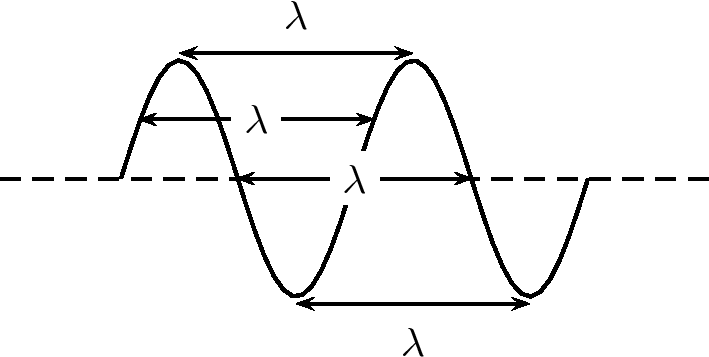
\includegraphics[width=300px]{col11305.imgs/m38806_PG10C5_011.png} % m38806;PG10C5\_011.png;;;6.0;8.5;
        
      \vspace{2pt}
    \vspace{.1in}
    
    \end{center}

 \end{figure}   

    \addtocounter{footnote}{-0}
    
        \par 
        \label{m38806*id319121}Points that are not in phase, those that are not separated by a complete number of wavelengths, are called \textsl{out of phase}. Examples of points like these would be \begin{math}A\end{math} and \begin{math}C\end{math}, or \begin{math}D\end{math} and \begin{math}E\end{math}, or \begin{math}B\end{math} and \begin{math}H\end{math} in the Activity.\par 
      
      \label{m38806*uid20}
            \subsection{ Period and Frequency}
            \nopagebreak
            
        
        \label{m38806*id319195}Imagine you are sitting next to a pond and you watch the waves going past you. First one peak arrives, then a trough, and then another peak. Suppose you measure the time taken between one peak arriving and then the next. This time will be the same for any two successive peaks passing you. We call this
time the \textsl{period}, and it is a characteristic of the wave.\par 
        \label{m38806*id319207}The symbol \begin{math}T\end{math} is used to represent the period. The period is measured in seconds (\begin{math}\mathrm{s}\end{math}).\par 
\label{m38806*fhsst!!!underscore!!!id426}\begin{definition}
	  \begin{tabular*}{15 cm}{m{15 mm}m{}}
	\hspace*{-50pt}  
\includegraphics[width=0.5in]{col11305.imgs/psflag2.png}   & \Definition{   \label{id2440606}\textbf{ Period (\begin{math}\mathrm{T}\end{math}) }} { \label{m38806*meaningfhsst!!!underscore!!!id426}The period (\begin{math}\mathrm{T}\end{math}) is the time taken for two successive peaks (or troughs) to pass a fixed point.
        
         } 
      \end{tabular*}
      \end{definition}

        \label{m38806*id319238}Imagine the pond again. Just as a peak passes you, you start your stopwatch and count each peak going past. After 1 second you stop the clock and stop counting. The number of peaks that you have counted in the 1 second is the \textsl{frequency} of the wave.\par 
\label{m38806*fhsst!!!underscore!!!id430}\begin{definition}
	  \begin{tabular*}{15 cm}{m{15 mm}m{}}
	\hspace*{-50pt}  
\includegraphics[width=0.5in]{col11305.imgs/psflag2.png}   & \Definition{   \label{id2440655}\textbf{ Frequency }} { \label{m38806*meaningfhsst!!!underscore!!!id430}
        The frequency is the number of successive peaks (or troughs) passing a given point in 1 second.
         } 
      \end{tabular*}
      \end{definition}

        \label{m38806*id319268}The frequency and the period are related to each other. As the period is the time taken for 1 peak to pass, then the number of peaks passing the point in 1 second is \begin{math}\frac{1}{T}\end{math}. But this is the frequency. So\par 
        \label{m38806*id319287}\nopagebreak\noindent{}
          \settowidth{\mymathboxwidth}{\begin{equation}
    f=\frac{1}{T}\tag{7.2}
      \end{equation}
    }
    \typeout{Columnwidth = \the\columnwidth}\typeout{math as usual width = \the\mymathboxwidth}
    \ifthenelse{\lengthtest{\mymathboxwidth < \columnwidth}}{% if the math fits, do it again, for real
    \begin{equation}
    f=\frac{1}{T}\tag{7.2}
      \end{equation}
    }{% else, if it doesn't fit
    \setlength{\mymathboxwidth}{\columnwidth}
      \addtolength{\mymathboxwidth}{-48pt}
    \par\vspace{12pt}\noindent\begin{minipage}{\columnwidth}
    \parbox[t]{\mymathboxwidth}{\large\begin{math}
    f=\frac{1}{T}\end{math}}\hfill
    \parbox[t]{48pt}{\raggedleft 
    (7.2)}
    \end{minipage}\vspace{12pt}\par
    }% end of conditional for this bit of math
    \typeout{math as usual width = \the\mymathboxwidth}
    
        
        \label{m38806*id319306}or alternatively,\par 
        \label{m38806*id319312}\nopagebreak\noindent{}\settowidth{\mymathboxwidth}{\begin{equation}
    T=\frac{1}{f}\tag{7.3}
      \end{equation}
    }
    \typeout{Columnwidth = \the\columnwidth}\typeout{math as usual width = \the\mymathboxwidth}
    \ifthenelse{\lengthtest{\mymathboxwidth < \columnwidth}}{% if the math fits, do it again, for real
    \begin{equation}
    T=\frac{1}{f}\tag{7.3}
      \end{equation}
    }{% else, if it doesn't fit
    \setlength{\mymathboxwidth}{\columnwidth}
      \addtolength{\mymathboxwidth}{-48pt}
    \par\vspace{12pt}\noindent\begin{minipage}{\columnwidth}
    \parbox[t]{\mymathboxwidth}{\large\begin{math}
    T=\frac{1}{f}\end{math}}\hfill
    \parbox[t]{48pt}{\raggedleft 
    (7.3)}
    \end{minipage}\vspace{12pt}\par
    }% end of conditional for this bit of math
    \typeout{math as usual width = \the\mymathboxwidth}
    
        
        \label{m38806*id319335}For example, if the time between two consecutive peaks passing a fixed point is \begin{math}\frac{1}{2}\phantom{\rule{0.166667em}{0ex}}\mathrm{s}\end{math}, then the period of the wave is \begin{math}\frac{1}{2}\phantom{\rule{0.166667em}{0ex}}\mathrm{s}\end{math}. Therefore, the frequency of the wave is:\par 
        \label{m38806*id319375}\nopagebreak\noindent{}\settowidth{\mymathboxwidth}{\begin{equation}
    \begin{array}{ccc}\hfill f& =& \frac{1}{T}\hfill \\ & =& \frac{1}{\frac{1}{2}\phantom{\rule{0.166667em}{0ex}}\mathrm{s}}\hfill \\ & =& 2\phantom{\rule{0.166667em}{0ex}}{\mathrm{s}}^{-1}\hfill \end{array}\tag{7.4}
      \end{equation}
    }
    \typeout{Columnwidth = \the\columnwidth}\typeout{math as usual width = \the\mymathboxwidth}
    \ifthenelse{\lengthtest{\mymathboxwidth < \columnwidth}}{% if the math fits, do it again, for real
    \begin{equation}
    \begin{array}{ccc}\hfill f& =& \frac{1}{T}\hfill \\ & =& \frac{1}{\frac{1}{2}\phantom{\rule{0.166667em}{0ex}}\mathrm{s}}\hfill \\ & =& 2\phantom{\rule{0.166667em}{0ex}}{\mathrm{s}}^{-1}\hfill \end{array}\tag{7.4}
      \end{equation}
    }{% else, if it doesn't fit
    \setlength{\mymathboxwidth}{\columnwidth}
      \addtolength{\mymathboxwidth}{-48pt}
    \par\vspace{12pt}\noindent\begin{minipage}{\columnwidth}
    \parbox[t]{\mymathboxwidth}{\large\begin{math}
    f=\frac{1}{T}=\frac{1}{\frac{1}{2}\phantom{\rule{0.166667em}{0ex}}\mathrm{s}}=2\phantom{\rule{0.166667em}{0ex}}{\mathrm{s}}^{-1}\end{math}}\hfill
    \parbox[t]{48pt}{\raggedleft 
    (7.4)}
    \end{minipage}\vspace{12pt}\par
    }% end of conditional for this bit of math
    \typeout{math as usual width = \the\mymathboxwidth}
    
        
        \label{m38806*id319462}The unit of frequency is the Hertz (\begin{math}\mathrm{Hz}\end{math}) or \begin{math}{\mathrm{s}}^{-1}\end{math}.\par 
\label{m38806*secfhsst!!!underscore!!!id520}\vspace{.5cm} 
      
      \noindent
      \hspace*{-30pt}
\includegraphics[width=0.5in]{col11305.imgs/pspencil2.png}   \raisebox{25mm}{   
      \begin{mdframed}[linewidth=4, leftmargin=40, rightmargin=40]  
      \begin{exercise}
    \noindent\textbf{Exercise 7.3:  Period and Frequency }
        \label{m38806*probfhsst!!!underscore!!!id521}
        \label{m38806*id319502}What is the period of a wave of frequency \begin{math}10\phantom{\rule{2pt}{0ex}}\mathrm{Hz}\end{math}? \par 
        \vspace{5pt}
        \label{m38806*solfhsst!!!underscore!!!id524}\noindent\textbf{Solution to Exercise } \label{m38806*listfhsst!!!underscore!!!id524}\begin{enumerate}[noitemsep, label=\textbf{Step} \textbf{\arabic*}. ] 
            \leftskip=20pt\rightskip=\leftskip\item  
        \label{m38806*id319526}We are required to calculate the period of a \begin{math}10\phantom{\rule{2pt}{0ex}}\mathrm{Hz}\end{math} wave.\par 
        \item  
        \label{m38806*id319534}We know that:\par 
        \label{m38806*id319538}\nopagebreak\noindent{}
          \settowidth{\mymathboxwidth}{\begin{equation}
    T=\frac{1}{f}\tag{7.5}
      \end{equation}
    }
    \typeout{Columnwidth = \the\columnwidth}\typeout{math as usual width = \the\mymathboxwidth}
    \ifthenelse{\lengthtest{\mymathboxwidth < \columnwidth}}{% if the math fits, do it again, for real
    \begin{equation}
    T=\frac{1}{f}\tag{7.5}
      \end{equation}
    }{% else, if it doesn't fit
    \setlength{\mymathboxwidth}{\columnwidth}
      \addtolength{\mymathboxwidth}{-48pt}
    \par\vspace{12pt}\noindent\begin{minipage}{\columnwidth}
    \parbox[t]{\mymathboxwidth}{\large\begin{math}
    T=\frac{1}{f}\end{math}}\hfill
    \parbox[t]{48pt}{\raggedleft 
    (7.5)}
    \end{minipage}\vspace{12pt}\par
    }% end of conditional for this bit of math
    \typeout{math as usual width = \the\mymathboxwidth}
    
        
        \item  
        \label{m38806*id319563}\nopagebreak\noindent{}
          \settowidth{\mymathboxwidth}{\begin{equation}
    \begin{array}{ccc}\hfill T& =& \frac{1}{f}\hfill \\ & =& \frac{1}{10\phantom{\rule{0.166667em}{0ex}}\mathrm{Hz}}\hfill \\ & =& 0,1\phantom{\rule{0.166667em}{0ex}}\mathrm{s}\hfill \end{array}\tag{7.6}
      \end{equation}
    }
    \typeout{Columnwidth = \the\columnwidth}\typeout{math as usual width = \the\mymathboxwidth}
    \ifthenelse{\lengthtest{\mymathboxwidth < \columnwidth}}{% if the math fits, do it again, for real
    \begin{equation}
    \begin{array}{ccc}\hfill T& =& \frac{1}{f}\hfill \\ & =& \frac{1}{10\phantom{\rule{0.166667em}{0ex}}\mathrm{Hz}}\hfill \\ & =& 0,1\phantom{\rule{0.166667em}{0ex}}\mathrm{s}\hfill \end{array}\tag{7.6}
      \end{equation}
    }{% else, if it doesn't fit
    \setlength{\mymathboxwidth}{\columnwidth}
      \addtolength{\mymathboxwidth}{-48pt}
    \par\vspace{12pt}\noindent\begin{minipage}{\columnwidth}
    \parbox[t]{\mymathboxwidth}{\large\begin{math}
    T=\frac{1}{f}=\frac{1}{10\phantom{\rule{0.166667em}{0ex}}\mathrm{Hz}}=0,1\phantom{\rule{0.166667em}{0ex}}\mathrm{s}\end{math}}\hfill
    \parbox[t]{48pt}{\raggedleft 
    (7.6)}
    \end{minipage}\vspace{12pt}\par
    }% end of conditional for this bit of math
    \typeout{math as usual width = \the\mymathboxwidth}
    
        
        \item  
        \label{m38806*id319644}The period of a \begin{math}10\phantom{\rule{2pt}{0ex}}\mathrm{Hz}\end{math} wave is \begin{math}0,1\phantom{\rule{2pt}{0ex}}\mathrm{s}\end{math}. \par 
        \end{enumerate}
         

    \end{exercise}
    \end{mdframed}
    }
    \noindent
  
      
      \label{m38806*uid21}
            \subsection{ Speed of a Transverse Wave}
            \nopagebreak
            
        
        \label{m38806*id319670}In Motion in One Dimension, we saw that speed was defined as\par 
        \label{m38806*id319676}\nopagebreak\noindent{}\settowidth{\mymathboxwidth}{\begin{equation}
    \mathrm{speed}=\frac{\mathrm{distance}\phantom{\rule{2pt}{0ex}}\mathrm{traveled}}{\mathrm{time}\phantom{\rule{2pt}{0ex}}\mathrm{taken}}\tag{7.7}
      \end{equation}
    }
    \typeout{Columnwidth = \the\columnwidth}\typeout{math as usual width = \the\mymathboxwidth}
    \ifthenelse{\lengthtest{\mymathboxwidth < \columnwidth}}{% if the math fits, do it again, for real
    \begin{equation}
    \mathrm{speed}=\frac{\mathrm{distance}\phantom{\rule{2pt}{0ex}}\mathrm{traveled}}{\mathrm{time}\phantom{\rule{2pt}{0ex}}\mathrm{taken}}\tag{7.7}
      \end{equation}
    }{% else, if it doesn't fit
    \setlength{\mymathboxwidth}{\columnwidth}
      \addtolength{\mymathboxwidth}{-48pt}
    \par\vspace{12pt}\noindent\begin{minipage}{\columnwidth}
    \parbox[t]{\mymathboxwidth}{\large\begin{math}
    \mathrm{speed}=\frac{\mathrm{distance}\phantom{\rule{2pt}{0ex}}\mathrm{traveled}}{\mathrm{time}\phantom{\rule{2pt}{0ex}}\mathrm{taken}}\end{math}}\hfill
    \parbox[t]{48pt}{\raggedleft 
    (7.7)}
    \end{minipage}\vspace{12pt}\par
    }% end of conditional for this bit of math
    \typeout{math as usual width = \the\mymathboxwidth}
    
        
        \label{m38806*id319706}The distance between two successive peaks is 1 wavelength, \begin{math}\lambda \end{math}. Thus in a time of 1 period, the wave will travel 1 wavelength in distance. Thus the speed of the wave, \begin{math}v\end{math}, is:\par 
        \label{m38806*id319732}\nopagebreak\noindent{}\settowidth{\mymathboxwidth}{\begin{equation}
    v=\frac{\text{distance}\phantom{\rule{4.pt}{0ex}}\text{traveled}}{\text{time}\phantom{\rule{4.pt}{0ex}}\text{taken}}=\frac{\lambda }{T}\tag{7.8}
      \end{equation}
    }
    \typeout{Columnwidth = \the\columnwidth}\typeout{math as usual width = \the\mymathboxwidth}
    \ifthenelse{\lengthtest{\mymathboxwidth < \columnwidth}}{% if the math fits, do it again, for real
    \begin{equation}
    v=\frac{\text{distance}\phantom{\rule{4.pt}{0ex}}\text{traveled}}{\text{time}\phantom{\rule{4.pt}{0ex}}\text{taken}}=\frac{\lambda }{T}\tag{7.8}
      \end{equation}
    }{% else, if it doesn't fit
    \setlength{\mymathboxwidth}{\columnwidth}
      \addtolength{\mymathboxwidth}{-48pt}
    \par\vspace{12pt}\noindent\begin{minipage}{\columnwidth}
    \parbox[t]{\mymathboxwidth}{\large\begin{math}
    v=\frac{\text{distance}\phantom{\rule{4.pt}{0ex}}\text{traveled}}{\text{time}\phantom{\rule{4.pt}{0ex}}\text{taken}}=\frac{\lambda }{T}\end{math}}\hfill
    \parbox[t]{48pt}{\raggedleft 
    (7.8)}
    \end{minipage}\vspace{12pt}\par
    }% end of conditional for this bit of math
    \typeout{math as usual width = \the\mymathboxwidth}
    
        
        \label{m38806*id319776}However, \begin{math}f=\frac{1}{T}\end{math}. Therefore, we can also write:\par 
        \label{m38806*id319802}\nopagebreak\noindent{}
          \settowidth{\mymathboxwidth}{\begin{equation}
    \begin{array}{ccc}\hfill v& =& \frac{\lambda }{T}\hfill \\ & =& \lambda \ensuremath{\cdot}\frac{1}{T}\hfill \\ & =& \lambda \ensuremath{\cdot}f\hfill \end{array}\tag{7.9}
      \end{equation}
    }
    \typeout{Columnwidth = \the\columnwidth}\typeout{math as usual width = \the\mymathboxwidth}
    \ifthenelse{\lengthtest{\mymathboxwidth < \columnwidth}}{% if the math fits, do it again, for real
    \begin{equation}
    \begin{array}{ccc}\hfill v& =& \frac{\lambda }{T}\hfill \\ & =& \lambda \ensuremath{\cdot}\frac{1}{T}\hfill \\ & =& \lambda \ensuremath{\cdot}f\hfill \end{array}\tag{7.9}
      \end{equation}
    }{% else, if it doesn't fit
    \setlength{\mymathboxwidth}{\columnwidth}
      \addtolength{\mymathboxwidth}{-48pt}
    \par\vspace{12pt}\noindent\begin{minipage}{\columnwidth}
    \parbox[t]{\mymathboxwidth}{\large\begin{math}
    v=\frac{\lambda }{T}=\lambda \ensuremath{\cdot}\frac{1}{T}=\lambda \ensuremath{\cdot}f\end{math}}\hfill
    \parbox[t]{48pt}{\raggedleft 
    (7.9)}
    \end{minipage}\vspace{12pt}\par
    }% end of conditional for this bit of math
    \typeout{math as usual width = \the\mymathboxwidth}
    
        
        \label{m38806*id319870}We call this equation the \textsl{wave equation}. To summarise, we have that \begin{math}v=\lambda \ensuremath{\cdot}f\end{math} where\par 
        \label{m38806*id319901}\begin{itemize}[noitemsep]
            \label{m38806*uid22}\item \begin{math}v=\end{math} speed in \begin{math}\mathrm{m}\ensuremath{\cdot}\mathrm{s}{}^{-1}\end{math}\label{m38806*uid23}\item \begin{math}\lambda =\end{math} wavelength in \begin{math}\mathrm{m}\end{math}
\label{m38806*uid24}\item \begin{math}f=\end{math} frequency in \begin{math}\mathrm{Hz}\end{math}
\end{itemize}
        
\par
            \label{m38806*secfhsst!!!underscore!!!id705}\vspace{.5cm} 
      
      \noindent
      \hspace*{-30pt}
\includegraphics[width=0.5in]{col11305.imgs/pspencil2.png}   \raisebox{25mm}{   
      \begin{mdframed}[linewidth=4, leftmargin=40, rightmargin=40]  
      \begin{exercise}
    \noindent\textbf{Exercise 7.4:  Speed of a Transverse Wave 1 }
        \label{m38806*probfhsst!!!underscore!!!id706}
        \label{m38806*id320001}When a particular string is vibrated at a frequency of \begin{math}10\phantom{\rule{2pt}{0ex}}\mathrm{Hz}\end{math}, a transverse wave of wavelength \begin{math}0,25\phantom{\rule{2pt}{0ex}}\mathrm{m}\end{math} is produced. Determine the speed of the wave as it travels along the string. \par 
        \vspace{5pt}
        \label{m38806*solfhsst!!!underscore!!!id709}\noindent\textbf{Solution to Exercise } \label{m38806*listfhsst!!!underscore!!!id709}\begin{enumerate}[noitemsep, label=\textbf{Step} \textbf{\arabic*}. ] 
            \leftskip=20pt\rightskip=\leftskip\item  
        \label{m38806*id320028}\begin{itemize}[noitemsep]
            \leftskip=20pt\rightskip=\leftskip\label{m38806*uid25}\item frequency of wave: \begin{math}f=10\mathrm{Hz}\end{math}
\label{m38806*uid26}\item wavelength of wave: \begin{math}\lambda =0,25\mathrm{m}\end{math}
\end{itemize}
        
        \label{m38806*id320081}We are required to calculate the speed of the wave as it travels along the string. All quantities are in SI units.\par 
        \item  
        \label{m38806*id320089}We know that the speed of a wave is:\par 
        \label{m38806*id320093}\nopagebreak\noindent{}
          \settowidth{\mymathboxwidth}{\begin{equation}
    v=f\ensuremath{\cdot}\lambda \tag{7.10}
      \end{equation}
    }
    \typeout{Columnwidth = \the\columnwidth}\typeout{math as usual width = \the\mymathboxwidth}
    \ifthenelse{\lengthtest{\mymathboxwidth < \columnwidth}}{% if the math fits, do it again, for real
    \begin{equation}
    v=f\ensuremath{\cdot}\lambda \tag{7.10}
      \end{equation}
    }{% else, if it doesn't fit
    \setlength{\mymathboxwidth}{\columnwidth}
      \addtolength{\mymathboxwidth}{-48pt}
    \par\vspace{12pt}\noindent\begin{minipage}{\columnwidth}
    \parbox[t]{\mymathboxwidth}{\large\begin{math}
    v=f\ensuremath{\cdot}\lambda \end{math}}\hfill
    \parbox[t]{48pt}{\raggedleft 
    (7.10)}
    \end{minipage}\vspace{12pt}\par
    }% end of conditional for this bit of math
    \typeout{math as usual width = \the\mymathboxwidth}
    
        
        \label{m38806*id320114}and we are given all the necessary quantities.\par 
        \item  
        \label{m38806*id320123}\nopagebreak\noindent{}
          \settowidth{\mymathboxwidth}{\begin{equation}
    \begin{array}{ccc}\hfill v& =& f\ensuremath{\cdot}\lambda \hfill \\ & =& \left(10\phantom{\rule{0.277778em}{0ex}}\mathrm{Hz}\right)\left(0,25\phantom{\rule{0.166667em}{0ex}}\mathrm{m}\right)\hfill \\ & =& 2,5\phantom{\rule{0.166667em}{0ex}}\mathrm{m}\ensuremath{\cdot}{\mathrm{s}}^{-1}\hfill \end{array}\tag{7.11}
      \end{equation}
    }
    \typeout{Columnwidth = \the\columnwidth}\typeout{math as usual width = \the\mymathboxwidth}
    \ifthenelse{\lengthtest{\mymathboxwidth < \columnwidth}}{% if the math fits, do it again, for real
    \begin{equation}
    \begin{array}{ccc}\hfill v& =& f\ensuremath{\cdot}\lambda \hfill \\ & =& \left(10\phantom{\rule{0.277778em}{0ex}}\mathrm{Hz}\right)\left(0,25\phantom{\rule{0.166667em}{0ex}}\mathrm{m}\right)\hfill \\ & =& 2,5\phantom{\rule{0.166667em}{0ex}}\mathrm{m}\ensuremath{\cdot}{\mathrm{s}}^{-1}\hfill \end{array}\tag{7.11}
      \end{equation}
    }{% else, if it doesn't fit
    \setlength{\mymathboxwidth}{\columnwidth}
      \addtolength{\mymathboxwidth}{-48pt}
    \par\vspace{12pt}\noindent\begin{minipage}{\columnwidth}
    \parbox[t]{\mymathboxwidth}{\large\begin{math}
    v=f\ensuremath{\cdot}\lambda =\left(10\phantom{\rule{0.277778em}{0ex}}\mathrm{Hz}\right)\left(0,25\phantom{\rule{0.166667em}{0ex}}\mathrm{m}\right)=2,5\phantom{\rule{0.166667em}{0ex}}\mathrm{m}\ensuremath{\cdot}{\mathrm{s}}^{-1}\end{math}}\hfill
    \parbox[t]{48pt}{\raggedleft 
    (7.11)}
    \end{minipage}\vspace{12pt}\par
    }% end of conditional for this bit of math
    \typeout{math as usual width = \the\mymathboxwidth}
    
        
        \item  
        \label{m38806*id320240}The wave travels at \begin{math}2,5\phantom{\rule{2pt}{0ex}}\mathrm{m}\ensuremath{\cdot}\mathrm{s}{}^{-1}\end{math} along the string.
 \par 
        \end{enumerate}
         

    \end{exercise}
    \end{mdframed}
    }
    \noindent
  
\label{m38806*secfhsst!!!underscore!!!id804}\vspace{.5cm} 
      
      \noindent
      \hspace*{-30pt}
\includegraphics[width=0.5in]{col11305.imgs/pspencil2.png}   \raisebox{25mm}{   
      \begin{mdframed}[linewidth=4, leftmargin=40, rightmargin=40]  
      \begin{exercise}
    \noindent\textbf{Exercise 7.5:  Speed of a Transverse Wave 2 }
        \label{m38806*probfhsst!!!underscore!!!id805}
        \label{m38806*id320294}A cork on the surface of a swimming pool bobs up and down once every second on some ripples. The ripples have a wavelength of \begin{math}20\phantom{\rule{2pt}{0ex}}\mathrm{cm}\end{math}. If the cork is \begin{math}2\phantom{\rule{2pt}{0ex}}\mathrm{m}\end{math} from the edge of the pool, how long does it take a ripple passing the cork to reach the edge? \par 
        \vspace{5pt}
        \label{m38806*solfhsst!!!underscore!!!id808}\noindent\textbf{Solution to Exercise } \label{m38806*listfhsst!!!underscore!!!id808}\begin{enumerate}[noitemsep, label=\textbf{Step} \textbf{\arabic*}. ] 
            \leftskip=20pt\rightskip=\leftskip\item  
        \label{m38806*id320322}We are given:\par 
        \label{m38806*id320325}\begin{itemize}[noitemsep]
            \leftskip=20pt\rightskip=\leftskip\label{m38806*uid27}\item frequency of wave: \begin{math}f=1\phantom{\rule{2pt}{0ex}}\mathrm{Hz}\end{math}
\label{m38806*uid28}\item wavelength of wave: \begin{math}\lambda =20\phantom{\rule{2pt}{0ex}}\mathrm{cm}\end{math}
\label{m38806*uid29}\item distance of cork from edge of pool: \begin{math}D\phantom{\rule{0.166667em}{0ex}}=2\phantom{\rule{2pt}{0ex}}\mathrm{m}\end{math}
\end{itemize}
        
        \label{m38806*id320406}We are required to determine the time it takes for a ripple to travel between the cork and the edge of the pool.\par 
        \label{m38806*id320410}The wavelength is not in SI units and should be converted.\par 
        \item  
        \label{m38806*id320418}The time taken for the ripple to reach the edge of the pool is obtained from:\par 
        \label{m38806*id320422}\nopagebreak\noindent{}\settowidth{\mymathboxwidth}{\begin{equation}
    t=\frac{D}{v}\phantom{\rule{4pt}{0ex}}\phantom{\rule{4pt}{0ex}}\phantom{\rule{4pt}{0ex}}\phantom{\rule{4pt}{0ex}}\phantom{\rule{4pt}{0ex}}\left(\text{from}\phantom{\rule{4pt}{0ex}}v=\frac{D}{t}\right)\tag{7.12}
      \end{equation}
    }
    \typeout{Columnwidth = \the\columnwidth}\typeout{math as usual width = \the\mymathboxwidth}
    \ifthenelse{\lengthtest{\mymathboxwidth < \columnwidth}}{% if the math fits, do it again, for real
    \begin{equation}
    t=\frac{D}{v}\phantom{\rule{4pt}{0ex}}\phantom{\rule{4pt}{0ex}}\phantom{\rule{4pt}{0ex}}\phantom{\rule{4pt}{0ex}}\phantom{\rule{4pt}{0ex}}\left(\text{from}\phantom{\rule{4pt}{0ex}}v=\frac{D}{t}\right)\tag{7.12}
      \end{equation}
    }{% else, if it doesn't fit
    \setlength{\mymathboxwidth}{\columnwidth}
      \addtolength{\mymathboxwidth}{-48pt}
    \par\vspace{12pt}\noindent\begin{minipage}{\columnwidth}
    \parbox[t]{\mymathboxwidth}{\large\begin{math}
    t=\frac{D}{v}\phantom{\rule{4pt}{0ex}}\phantom{\rule{4pt}{0ex}}\phantom{\rule{4pt}{0ex}}\phantom{\rule{4pt}{0ex}}\phantom{\rule{4pt}{0ex}}\left(\text{from}\phantom{\rule{4pt}{0ex}}v=\frac{D}{t}\right)\end{math}}\hfill
    \parbox[t]{48pt}{\raggedleft 
    (7.12)}
    \end{minipage}\vspace{12pt}\par
    }% end of conditional for this bit of math
    \typeout{math as usual width = \the\mymathboxwidth}
    
        
        \label{m38806*id320480}We know that\par 
        \label{m38806*id320485}\nopagebreak\noindent{}
          \settowidth{\mymathboxwidth}{\begin{equation}
    v=f\ensuremath{\cdot}\lambda \tag{7.13}
      \end{equation}
    }
    \typeout{Columnwidth = \the\columnwidth}\typeout{math as usual width = \the\mymathboxwidth}
    \ifthenelse{\lengthtest{\mymathboxwidth < \columnwidth}}{% if the math fits, do it again, for real
    \begin{equation}
    v=f\ensuremath{\cdot}\lambda \tag{7.13}
      \end{equation}
    }{% else, if it doesn't fit
    \setlength{\mymathboxwidth}{\columnwidth}
      \addtolength{\mymathboxwidth}{-48pt}
    \par\vspace{12pt}\noindent\begin{minipage}{\columnwidth}
    \parbox[t]{\mymathboxwidth}{\large\begin{math}
    v=f\ensuremath{\cdot}\lambda \end{math}}\hfill
    \parbox[t]{48pt}{\raggedleft 
    (7.13)}
    \end{minipage}\vspace{12pt}\par
    }% end of conditional for this bit of math
    \typeout{math as usual width = \the\mymathboxwidth}
    
        
        \label{m38806*id320506}Therefore,\par 
        \label{m38806*id320512}\nopagebreak\noindent{}\settowidth{\mymathboxwidth}{\begin{equation}
    t=\frac{D}{f\ensuremath{\cdot}\lambda }\tag{7.14}
      \end{equation}
    }
    \typeout{Columnwidth = \the\columnwidth}\typeout{math as usual width = \the\mymathboxwidth}
    \ifthenelse{\lengthtest{\mymathboxwidth < \columnwidth}}{% if the math fits, do it again, for real
    \begin{equation}
    t=\frac{D}{f\ensuremath{\cdot}\lambda }\tag{7.14}
      \end{equation}
    }{% else, if it doesn't fit
    \setlength{\mymathboxwidth}{\columnwidth}
      \addtolength{\mymathboxwidth}{-48pt}
    \par\vspace{12pt}\noindent\begin{minipage}{\columnwidth}
    \parbox[t]{\mymathboxwidth}{\large\begin{math}
    t=\frac{D}{f\ensuremath{\cdot}\lambda }\end{math}}\hfill
    \parbox[t]{48pt}{\raggedleft 
    (7.14)}
    \end{minipage}\vspace{12pt}\par
    }% end of conditional for this bit of math
    \typeout{math as usual width = \the\mymathboxwidth}
    
        
        \item  
        \label{m38806*id320542}\nopagebreak\noindent{}
          \settowidth{\mymathboxwidth}{\begin{equation}
    20\phantom{\rule{0.166667em}{0ex}}\mathrm{cm}=0,2\phantom{\rule{0.166667em}{0ex}}\mathrm{m}\tag{7.15}
      \end{equation}
    }
    \typeout{Columnwidth = \the\columnwidth}\typeout{math as usual width = \the\mymathboxwidth}
    \ifthenelse{\lengthtest{\mymathboxwidth < \columnwidth}}{% if the math fits, do it again, for real
    \begin{equation}
    20\phantom{\rule{0.166667em}{0ex}}\mathrm{cm}=0,2\phantom{\rule{0.166667em}{0ex}}\mathrm{m}\tag{7.15}
      \end{equation}
    }{% else, if it doesn't fit
    \setlength{\mymathboxwidth}{\columnwidth}
      \addtolength{\mymathboxwidth}{-48pt}
    \par\vspace{12pt}\noindent\begin{minipage}{\columnwidth}
    \parbox[t]{\mymathboxwidth}{\large\begin{math}
    20\phantom{\rule{0.166667em}{0ex}}\mathrm{cm}=0,2\phantom{\rule{0.166667em}{0ex}}\mathrm{m}\end{math}}\hfill
    \parbox[t]{48pt}{\raggedleft 
    (7.15)}
    \end{minipage}\vspace{12pt}\par
    }% end of conditional for this bit of math
    \typeout{math as usual width = \the\mymathboxwidth}
    
        
        \item  
        \label{m38806*id320580}\nopagebreak\noindent{}\settowidth{\mymathboxwidth}{\begin{equation}
    \begin{array}{ccc}\hfill t& =& \frac{D}{f\ensuremath{\cdot}\lambda }\hfill \\ & =& \frac{2\phantom{\rule{0.166667em}{0ex}}\mathrm{m}}{\left(1\phantom{\rule{0.277778em}{0ex}}\mathrm{Hz}\right)\left(0,2\phantom{\rule{0.166667em}{0ex}}\mathrm{m}\right)}\hfill \\ & =& 10\phantom{\rule{0.166667em}{0ex}}\mathrm{s}\hfill \end{array}\tag{7.16}
      \end{equation}
    }
    \typeout{Columnwidth = \the\columnwidth}\typeout{math as usual width = \the\mymathboxwidth}
    \ifthenelse{\lengthtest{\mymathboxwidth < \columnwidth}}{% if the math fits, do it again, for real
    \begin{equation}
    \begin{array}{ccc}\hfill t& =& \frac{D}{f\ensuremath{\cdot}\lambda }\hfill \\ & =& \frac{2\phantom{\rule{0.166667em}{0ex}}\mathrm{m}}{\left(1\phantom{\rule{0.277778em}{0ex}}\mathrm{Hz}\right)\left(0,2\phantom{\rule{0.166667em}{0ex}}\mathrm{m}\right)}\hfill \\ & =& 10\phantom{\rule{0.166667em}{0ex}}\mathrm{s}\hfill \end{array}\tag{7.16}
      \end{equation}
    }{% else, if it doesn't fit
    \setlength{\mymathboxwidth}{\columnwidth}
      \addtolength{\mymathboxwidth}{-48pt}
    \par\vspace{12pt}\noindent\begin{minipage}{\columnwidth}
    \parbox[t]{\mymathboxwidth}{\large\begin{math}
    t=\frac{D}{f\ensuremath{\cdot}\lambda }=\frac{2\phantom{\rule{0.166667em}{0ex}}\mathrm{m}}{\left(1\phantom{\rule{0.277778em}{0ex}}\mathrm{Hz}\right)\left(0,2\phantom{\rule{0.166667em}{0ex}}\mathrm{m}\right)}=10\phantom{\rule{0.166667em}{0ex}}\mathrm{s}\end{math}}\hfill
    \parbox[t]{48pt}{\raggedleft 
    (7.16)}
    \end{minipage}\vspace{12pt}\par
    }% end of conditional for this bit of math
    \typeout{math as usual width = \the\mymathboxwidth}
    
        
        \item  
        \label{m38806*id320694}A ripple passing the leaf will take \begin{math}10\phantom{\rule{2pt}{0ex}}\mathrm{s}\end{math} to reach the edge of the pool. \par 
        \end{enumerate}
         

    \end{exercise}
    \end{mdframed}
    }
    \noindent
  
\label{m38806*eip-872}The following video provides a summary of the concepts covered so far.

    \setcounter{subfigure}{0}


	\begin{figure}[H] % horizontal\label{m38806*waves-1}
    
    
    \textnormal{Khan academy video on waves - 1}\vspace{.1in} \nopagebreak
  \label{m38806*yt-media1}\label{m38806*yt-video1}
            \raisebox{-5 pt}{ 
\includegraphics[width=0.5cm]{col11305.imgs/summary_www.png}} { (Video:  P10043 )}
      
      \vspace{2pt}
    \vspace{.1in}
    
    

 \end{figure}   

    \addtocounter{footnote}{-0}
    \par \label{m38806*secfhsst!!!underscore!!!id968}
            \subsubsection{ Waves }
            \nopagebreak
            \label{m38806*id320717}\begin{enumerate}[noitemsep, label=\textbf{\arabic*}. ] 
            \label{m38806*uid30}\item When the particles of a medium move perpendicular to the direction of the wave motion, the wave is called a \begin{math}.........\end{math} wave.\newline
            
\label{m38806*uid31}\item A transverse wave is moving downwards. In what direction do the particles in the medium move?\newline
            
\label{m38806*uid32}\item Consider the diagram below and answer the questions that follow:

    \setcounter{subfigure}{0}


	\begin{figure}[H] % horizontal\label{m38806*id320776}
    \begin{center}
    \label{m38806*id320776!!!underscore!!!media}\label{m38806*id320776!!!underscore!!!printimage}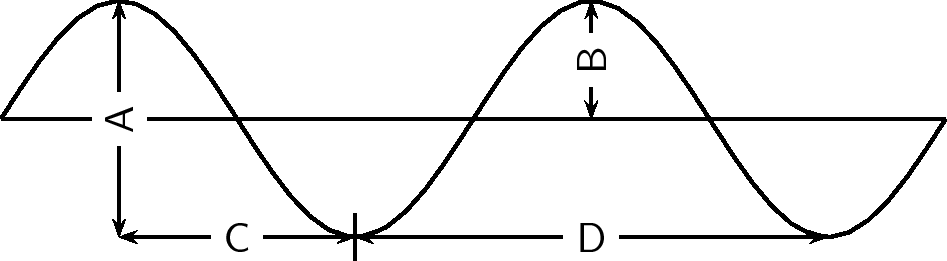
\includegraphics[width=300px]{col11305.imgs/m38806_PG10C5_012.png} % m38806;PG10C5\_012.png;;;6.0;8.5;
        
      \vspace{2pt}
    \vspace{.1in}
    
    \end{center}

 \end{figure}   

    \addtocounter{footnote}{-0}
    \label{m38806*id320783}\begin{enumerate}[noitemsep, label=\textbf{\alph*}. ] 
            \label{m38806*uid33}\item the wavelength of the wave is shown by letter \uline{\hspace{10ex}}.
\label{m38806*uid34}\item the amplitude of the wave is shown by letter \uline{\hspace{10ex}}.
\end{enumerate}
                \label{m38806*uid35}\item Draw 2 wavelengths of the following transverse waves on the same graph paper. Label all important values.
\label{m38806*id320849}\begin{enumerate}[noitemsep, label=\textbf{\alph*}. ] 
            \label{m38806*uid36}\item Wave 1: Amplitude = 1~cm, wavelength = 3~cm
\label{m38806*uid37}\item Wave 2: Peak to trough distance (vertical) = 3~cm, peak to peak distance (horizontal) = 5~cm
\end{enumerate}
                \label{m38806*uid38}\item You are given the transverse wave below.

    \setcounter{subfigure}{0}


	\begin{figure}[H] % horizontal\label{m38806*id320895}
    \begin{center}
    \label{m38806*id320895!!!underscore!!!media}\label{m38806*id320895!!!underscore!!!printimage}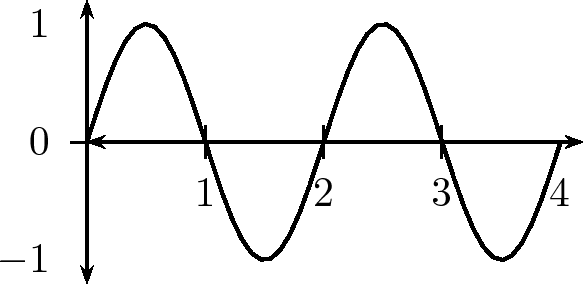
\includegraphics[width=300px]{col11305.imgs/m38806_PG10C5_013.png} % m38806;PG10C5\_013.png;;;6.0;8.5;
        
      \vspace{2pt}
    \vspace{.1in}
    
    \end{center}

 \end{figure}   

    \addtocounter{footnote}{-0}
    
Draw the following:
\label{m38806*id320905}\begin{enumerate}[noitemsep, label=\textbf{\alph*}. ] 
            \label{m38806*uid39}\item A wave with twice the amplitude of the given wave.
\label{m38806*uid40}\item A wave with half the amplitude of the given wave.
\label{m38806*uid41}\item A wave travelling at the same speed with twice the frequency of the given wave.
\label{m38806*uid42}\item A wave travelling at the same speed with half the frequency of the given wave.
\label{m38806*uid43}\item A wave with twice the wavelength of the given wave.
\label{m38806*uid44}\item A wave with half the wavelength of the given wave.
\label{m38806*uid45}\item A wave travelling at the same speed with twice the period of the given wave.
\label{m38806*uid46}\item A wave travelling at the same speed with half the period of the given wave.
\end{enumerate}
                \label{m38806*uid47}\item A transverse wave travelling at the same speed with an amplitude of 5~cm has a frequency of 15~Hz. The horizontal distance from a crest to the nearest trough is measured to be 2,5~cm. Find the
\label{m38806*id321026}\begin{enumerate}[noitemsep, label=\textbf{\alph*}. ] 
            \label{m38806*uid48}\item period of the wave.
\label{m38806*uid49}\item speed of the wave.
\end{enumerate}
                \label{m38806*uid50}\item A fly flaps its wings back and forth 200 times each second. Calculate the period of a wing flap.\newline
            
\label{m38806*uid51}\item As the period of a wave increases, the frequency 
\textsl{\textbf{increases/decreases/does not change.}}\newline
            
\label{m38806*uid52}\item Calculate the frequency of rotation of the second hand on a clock.\newline
            
\label{m38806*uid53}\item Microwave ovens produce radiation with a frequency of 2 450~MHz (1~MHz = \begin{math}{10}^{6}\end{math}~Hz) and a wavelength of 0,122~m. What is the wave speed of the radiation?\newline
            
\label{m38806*uid54}\item Study the following diagram and answer the questions:

    \setcounter{subfigure}{0}


	\begin{figure}[H] % horizontal\label{m38806*id321151}
    \begin{center}
    \label{m38806*id321151!!!underscore!!!media}\label{m38806*id321151!!!underscore!!!printimage}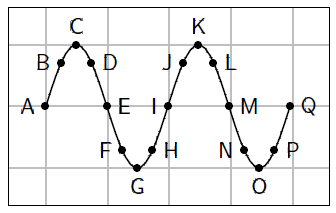
\includegraphics[width=300px]{col11305.imgs/m38806_PG10C5_014.png} % m38806;PG10C5\_014.png;;;6.0;8.5;
        
      \vspace{2pt}
    \vspace{.1in}
    
    \end{center}

 \end{figure}   

    \addtocounter{footnote}{-0}
    \label{m38806*id321157}\begin{enumerate}[noitemsep, label=\textbf{\alph*}. ] 
            \label{m38806*uid55}\item Identify two sets of points that are in phase.
\label{m38806*uid56}\item Identify two sets of points that are out of phase.
\label{m38806*uid57}\item Identify any two points that would indicate a wavelength.
\end{enumerate}
                \label{m38806*uid58}\item Tom is fishing from a pier and notices that four wave crests pass by in 8~s and estimates the distance between two successive crests is 4~m. The timing starts with the first crest and ends with the fourth. Calculate the speed of the wave.\newline
            
\end{enumerate}
        
        

      
    
\par \raisebox{-5 pt}{
\includegraphics[width=0.5cm]{col11305.imgs/summary_www.png}} Find the answers with the shortcodes:
 \par \begin{tabular}[h]{cccccc}
 (1.) liq  &  (2.) li4  &  (3.) li2  &  (4.) lr8  &  (5.) lr9  &  (6.) lrX  &  (7.) lrl  &  (8.) lr5  &  (9.) lrN  &  (10.) lrR  &  (11.) lrn  &  (12.) lrQ  & \end{tabular}



    \section{ Summary}
            \nopagebreak
            \label{m38806*cid6} $ \hspace{-5pt}\begin{array}{cccccccccccc}   \end{array} $ \hspace{2 pt}\raisebox{-5 pt}{
\includegraphics[width=0.5cm]{col11305.imgs/summary_www.png}} {(section shortcode: P10044 )} \par 
      
      \label{m38806*id324089}\begin{enumerate}[noitemsep, label=\textbf{\arabic*}. ] 
            \label{m38806*uid108}\item A wave is formed when a continuous number of pulses are transmitted through a medium.
\label{m38806*uid109}\item A peak is the highest point a particle in the medium rises to.
\label{m38806*uid110}\item A trough is the lowest point a particle in the medium sinks to.
\label{m38806*uid111}\item In a transverse wave, the particles move perpendicular to the motion of the wave.
\label{m38806*uid112}\item The amplitude is the maximum distance from equilibrium position to a peak (or trough), or the maximum displacement of a particle in a wave from its position of rest.
\label{m38806*uid113}\item The wavelength (\begin{math}\lambda \end{math}) is the distance between any two adjacent points on a wave that are in phase. It is measured in metres.
\label{m38806*uid114}\item The period (\begin{math}T\end{math}) of a wave is the time it takes a wavelength to pass a fixed point. It is measured in seconds (s).
\label{m38806*uid115}\item The frequency (\begin{math}f\end{math}) of a wave is how many waves pass a point in a second. It is measured in hertz (Hz) or \begin{math}\mathrm{s}{}^{-1}\end{math}.
\label{m38806*uid116}\item Frequency: \begin{math}f=\frac{1}{T}\end{math}\label{m38806*uid117}\item Period: \begin{math}T=\frac{1}{f}\end{math}\label{m38806*uid118}\item Speed: \begin{math}v=f\lambda \end{math} or \begin{math}v=\frac{\lambda }{T}\end{math}.
\label{m38806*uid119}\item When a wave is reflected from a fixed end, the resulting wave will move back through the medium, but will be inverted. When a wave is reflected from a free end, the waves are reflected, but not inverted.
\end{enumerate}
        
    
    \section{ Exercises}
            \nopagebreak
            \label{m38806*cid7} $ \hspace{-5pt}\begin{array}{cccccccccccc}   \end{array} $ \hspace{2 pt}\raisebox{-5 pt}{
\includegraphics[width=0.5cm]{col11305.imgs/summary_www.png}} {(section shortcode: P10045 )} \par 
      
      \label{m38806*id324367}\begin{enumerate}[noitemsep, label=\textbf{\arabic*}. ] 
            \label{m38806*uid120}\item A standing wave is formed when:
\label{m38806*id324383}\begin{enumerate}[noitemsep, label=\textbf{\alph*}. ] 
            \label{m38806*uid121}\item a wave refracts due to changes in the properties of the medium
\label{m38806*uid122}\item a wave reflects off a canyon wall and is heard shortly after it is formed
\label{m38806*uid123}\item a wave refracts and reflects due to changes in the medium
\label{m38806*uid124}\item two identical waves moving different directions along the same medium interfere
\end{enumerate}
                \label{m38806*uid125}\item How many nodes and anti-nodes are shown in the diagram?

    \setcounter{subfigure}{0}


	\begin{figure}[H] % horizontal\label{m38806*id324454}
    \begin{center}
    \label{m38806*id324454!!!underscore!!!media}\label{m38806*id324454!!!underscore!!!printimage}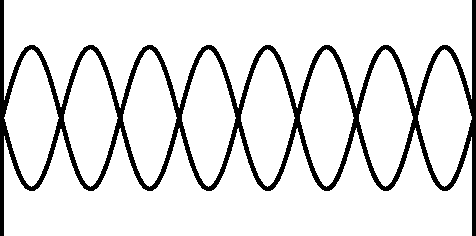
\includegraphics{col11305.imgs/m38806_PG10C5_049.png} % m38806;PG10C5\_049.png;;;6.0;8.5;
        
      \vspace{2pt}
    \vspace{.1in}
    
    \end{center}

 \end{figure}   

    \addtocounter{footnote}{-0}
            \label{m38806*uid126}\item Draw a transverse wave that is reflected from a fixed end.\newline
            
\label{m38806*uid127}\item Draw a transverse wave that is reflected from a free end.\newline
            
\label{m38806*uid128}\item A wave travels along a string at a speed of \begin{math}1,5\mathrm{m}\ensuremath{\cdot}\mathrm{s}{}^{-1}\end{math}. If the frequency of the source of the wave is 7,5 Hz, calculate:
\label{m38806*id324525}\begin{enumerate}[noitemsep, label=\textbf{\alph*}. ] 
            \label{m38806*uid129}\item the wavelength of the wave
\label{m38806*uid130}\item the period of the wave
\end{enumerate}
                \item Water waves crash against a seawall around the harbour. Eight waves hit the seawall in 5 s. The distance between successive troughs is 9 m. The height of the waveform trough to crest is 1,5 m. 
    \setcounter{subfigure}{0}


	\begin{figure}[H] % horizontal\label{m38806*id634524}
    \begin{center}
    \label{m38806*id634524!!!underscore!!!media}\label{m38806*id634524!!!underscore!!!printimage}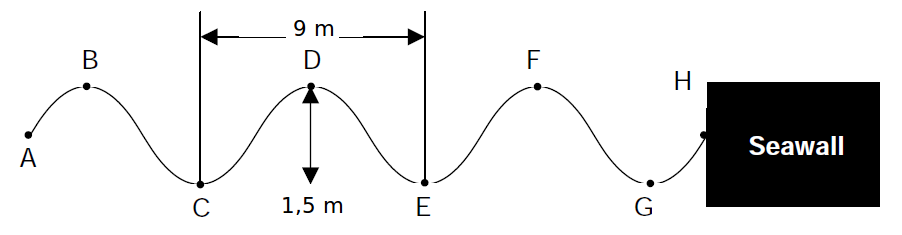
\includegraphics[width=0.8\columnwidth]{col11305.imgs/m38806_seawall.png} % m38806;seawall.png;;;6.0;8.5;
        
      \vspace{2pt}
    \vspace{.1in}
    
    \end{center}

 \end{figure}   

    \addtocounter{footnote}{-0}
    
\label{m38806*uid081231}\begin{enumerate}[noitemsep, label=\textbf{\alph*}. ] 
            \item How many complete waves are indicated in the sketch?\item Write down the letters that indicate any TWO points that are:
\label{m38806*uid0821323}\begin{enumerate}[noitemsep, label=\textbf{\roman*}. ] 
            \item in phase\item out of phase\item Represent ONE wavelength.\end{enumerate}
        \item Calculate the amplitude of the wave.\item Show that the period of the wave is 0,67 s.\item Calculate the frequency of the waves.\item Calculate the velocity of the waves.\end{enumerate}
        
         \end{enumerate}
        
    

  \label{m38806**end}
    
\par \raisebox{-5 pt}{
\includegraphics[width=0.5cm]{col11305.imgs/summary_www.png}} Find the answers with the shortcodes:
 \par \begin{tabular}[h]{cccccc}
 (1.) lrV  &  (2.) lrp  &  (3.) lrd  &  (4.) lrv  &  (5.) lrw  &  (6.) lrf  & \end{tabular}



